% Options for packages loaded elsewhere
\PassOptionsToPackage{unicode,pdfwindowui,pdfpagemode=FullScreen}{hyperref}
\PassOptionsToPackage{hyphens}{url}
\PassOptionsToPackage{dvipsnames,svgnames,x11names}{xcolor}
%
\documentclass[
  12pt,
  letterpaper,
]{article}

\usepackage{amsmath,amssymb}
\usepackage{setspace}
\usepackage{iftex}
\ifPDFTeX
  \usepackage[T1]{fontenc}
  \usepackage[utf8]{inputenc}
  \usepackage{textcomp} % provide euro and other symbols
\else % if luatex or xetex
  \usepackage{unicode-math}
  \defaultfontfeatures{Scale=MatchLowercase}
  \defaultfontfeatures[\rmfamily]{Ligatures=TeX,Scale=1}
\fi
\usepackage{lmodern}
\ifPDFTeX\else  
    % xetex/luatex font selection
    \setmainfont[]{TeX Gyre Pagella}
  \setmathfont[]{TeX Gyre Pagella Math}
\fi
% Use upquote if available, for straight quotes in verbatim environments
\IfFileExists{upquote.sty}{\usepackage{upquote}}{}
\IfFileExists{microtype.sty}{% use microtype if available
  \usepackage[]{microtype}
  \UseMicrotypeSet[protrusion]{basicmath} % disable protrusion for tt fonts
}{}
\makeatletter
\@ifundefined{KOMAClassName}{% if non-KOMA class
  \IfFileExists{parskip.sty}{%
    \usepackage{parskip}
  }{% else
    \setlength{\parindent}{0pt}
    \setlength{\parskip}{6pt plus 2pt minus 1pt}}
}{% if KOMA class
  \KOMAoptions{parskip=half}}
\makeatother
\usepackage{xcolor}
\usepackage[margin=1in]{geometry}
\setlength{\emergencystretch}{3em} % prevent overfull lines
\setcounter{secnumdepth}{-\maxdimen} % remove section numbering


\providecommand{\tightlist}{%
  \setlength{\itemsep}{0pt}\setlength{\parskip}{0pt}}\usepackage{longtable,booktabs,array}
\usepackage{calc} % for calculating minipage widths
% Correct order of tables after \paragraph or \subparagraph
\usepackage{etoolbox}
\makeatletter
\patchcmd\longtable{\par}{\if@noskipsec\mbox{}\fi\par}{}{}
\makeatother
% Allow footnotes in longtable head/foot
\IfFileExists{footnotehyper.sty}{\usepackage{footnotehyper}}{\usepackage{footnote}}
\makesavenoteenv{longtable}
\usepackage{graphicx}
\makeatletter
\newsavebox\pandoc@box
\newcommand*\pandocbounded[1]{% scales image to fit in text height/width
  \sbox\pandoc@box{#1}%
  \Gscale@div\@tempa{\textheight}{\dimexpr\ht\pandoc@box+\dp\pandoc@box\relax}%
  \Gscale@div\@tempb{\linewidth}{\wd\pandoc@box}%
  \ifdim\@tempb\p@<\@tempa\p@\let\@tempa\@tempb\fi% select the smaller of both
  \ifdim\@tempa\p@<\p@\scalebox{\@tempa}{\usebox\pandoc@box}%
  \else\usebox{\pandoc@box}%
  \fi%
}
% Set default figure placement to htbp
\def\fps@figure{htbp}
\makeatother
% definitions for citeproc citations
\NewDocumentCommand\citeproctext{}{}
\NewDocumentCommand\citeproc{mm}{%
  \begingroup\def\citeproctext{#2}\cite{#1}\endgroup}
\makeatletter
 % allow citations to break across lines
 \let\@cite@ofmt\@firstofone
 % avoid brackets around text for \cite:
 \def\@biblabel#1{}
 \def\@cite#1#2{{#1\if@tempswa , #2\fi}}
\makeatother
\newlength{\cslhangindent}
\setlength{\cslhangindent}{1.5em}
\newlength{\csllabelwidth}
\setlength{\csllabelwidth}{3em}
\newenvironment{CSLReferences}[2] % #1 hanging-indent, #2 entry-spacing
 {\begin{list}{}{%
  \setlength{\itemindent}{0pt}
  \setlength{\leftmargin}{0pt}
  \setlength{\parsep}{0pt}
  % turn on hanging indent if param 1 is 1
  \ifodd #1
   \setlength{\leftmargin}{\cslhangindent}
   \setlength{\itemindent}{-1\cslhangindent}
  \fi
  % set entry spacing
  \setlength{\itemsep}{#2\baselineskip}}}
 {\end{list}}
\usepackage{calc}
\newcommand{\CSLBlock}[1]{\hfill\break\parbox[t]{\linewidth}{\strut\ignorespaces#1\strut}}
\newcommand{\CSLLeftMargin}[1]{\parbox[t]{\csllabelwidth}{\strut#1\strut}}
\newcommand{\CSLRightInline}[1]{\parbox[t]{\linewidth - \csllabelwidth}{\strut#1\strut}}
\newcommand{\CSLIndent}[1]{\hspace{\cslhangindent}#1}

% -----------------------
% CUSTOM PREAMBLE STUFF
% -----------------------

% -----------------
% Title block stuff
% -----------------

% Abstract
\usepackage[runin]{abstract}
\renewcommand{\abstractnamefont}{\sffamily\small\bfseries}
\renewcommand{\abstracttextfont}{\sffamily\small}
\setlength{\absleftindent}{5pt}
\setlength{\absrightindent}{\absleftindent}

% Title
\usepackage{titling}
\pretitle{\par\begin{flushleft}\LARGE\sffamily\bfseries}
\posttitle{\par\end{flushleft}\vskip 10pt}

% Keywords
\newenvironment{keywords}
{\small\sffamily{\sffamily\small\bfseries{Keywords.}}}

% Authors
\usepackage{orcidlink}  % Create automatic ORCID icons/links
%\renewcommand{\and}{\end{tabular} \hskip 3em \begin{tabular}[t]{@{\hspace{0em}}l@{}}}
\preauthor{\begin{flushleft}
           \lineskip 1.5em}
\postauthor{\end{flushleft}}

% ------------------
% Section headings
% ------------------
\usepackage{titlesec}
\titleformat*{\section}{\Large\sffamily\bfseries\raggedright}
\titleformat*{\subsection}{\large\sffamily\bfseries\raggedright}
\titleformat*{\subsubsection}{\normalsize\sffamily\bfseries\raggedright}
\titleformat*{\paragraph}{\small\sffamily\bfseries\raggedright}

%\titlespacing{<command>}{<left>}{<before-sep>}{<after-sep>}
% Starred version removes indentation in following paragraph
\titlespacing*{\section}{0em}{2em}{0.1em}
\titlespacing*{\subsection}{0em}{1.25em}{0.1em}
\titlespacing*{\subsubsection}{0em}{0.75em}{0em}

% ------------------
% Headers/Footers
% ------------------
\usepackage{fancyhdr}
\pagestyle{fancy}
\fancyhf{}
\fancyhead[L,C,R]{}
\fancyfoot[L,C]{}
\fancyfoot[R]{\thepage}
\renewcommand{\headrulewidth}{1pt}
\fancypagestyle{plain}{%
    \renewcommand{\headrulewidth}{0pt}%
    \fancyhf{}%
    \fancyfoot[R]{\thepage}%
}
\renewcommand\footnoterule{\rule{\linewidth}{0.1pt}\vspace{5pt}}

% ------------------
% Captions
% ------------------
\usepackage[labelfont=bf,labelsep=period]{caption}
\captionsetup[figure]{font=footnotesize,justification=raggedright,singlelinecheck=false,format=hang}


% ---------------------------
% END CUSTOM PREAMBLE STUFF
% ---------------------------
\usepackage{booktabs}
\usepackage{longtable}
\usepackage{array}
\usepackage{multirow}
\usepackage{wrapfig}
\usepackage{float}
\usepackage{colortbl}
\usepackage{pdflscape}
\usepackage{tabu}
\usepackage{threeparttable}
\usepackage{threeparttablex}
\usepackage[normalem]{ulem}
\usepackage{makecell}
\usepackage{xcolor}
\usepackage{dcolumn} 
\makeatletter
\@ifpackageloaded{caption}{}{\usepackage{caption}}
\AtBeginDocument{%
\ifdefined\contentsname
  \renewcommand*\contentsname{Table of contents}
\else
  \newcommand\contentsname{Table of contents}
\fi
\ifdefined\listfigurename
  \renewcommand*\listfigurename{List of Figures}
\else
  \newcommand\listfigurename{List of Figures}
\fi
\ifdefined\listtablename
  \renewcommand*\listtablename{List of Tables}
\else
  \newcommand\listtablename{List of Tables}
\fi
\ifdefined\figurename
  \renewcommand*\figurename{Figure}
\else
  \newcommand\figurename{Figure}
\fi
\ifdefined\tablename
  \renewcommand*\tablename{Table}
\else
  \newcommand\tablename{Table}
\fi
}
\@ifpackageloaded{float}{}{\usepackage{float}}
\floatstyle{ruled}
\@ifundefined{c@chapter}{\newfloat{codelisting}{h}{lop}}{\newfloat{codelisting}{h}{lop}[chapter]}
\floatname{codelisting}{Listing}
\newcommand*\listoflistings{\listof{codelisting}{List of Listings}}
\makeatother
\makeatletter
\makeatother
\makeatletter
\@ifpackageloaded{caption}{}{\usepackage{caption}}
\@ifpackageloaded{subcaption}{}{\usepackage{subcaption}}
\makeatother

\usepackage{bookmark}

\IfFileExists{xurl.sty}{\usepackage{xurl}}{} % add URL line breaks if available
\urlstyle{same} % disable monospaced font for URLs
\hypersetup{
  pdftitle={title},
  colorlinks=true,
  linkcolor={blue},
  filecolor={Maroon},
  citecolor={Blue},
  urlcolor={RoyalBlue},
  pdfcreator={LaTeX via pandoc}}



\title{title}
% subtitles do not seem to work with article class?
%%\usepackage{etoolbox}
%\makeatletter
%\providecommand{\subtitle}[1]{% add subtitle to \maketitle
%  \apptocmd{\@title}{\par {\large #1 \par}}{}{}
%}
%\makeatother
%%\subtitle{subtitle}

\author{
{\bfseries \normalsize Isaiah Espinoza}%
 \\%
 \small University of Maryland, Department of Government and
Politics \\%
{\footnotesize \url{gespinoz@umd.edu}} \\\vspace{10pt}
}

\predate{}
\postdate{}
\date{}
\begin{document}

% for some reason this does not work in header
\renewcommand{\abstractname}{Abstract.}

% add the short title to the fancy header
\fancyhead[R]{A Short title}
\fancyhead[L]{Isaiah}

\maketitle
%\noindent \rule{\linewidth}{.5pt}
%\noindent \rule{\linewidth}{.5pt}


\setstretch{1.25}
\pagebreak

\subsection{Introduction}\label{introduction}

Election administration officials make efforts to sustain public trust
and confidence in the fairness and accuracy of elections, and attempt to
boost such confidence where it may be deprived. Concerns for safety have
developed among election staff and voters in more recent elections.
Regular measures are taken to enhance the
\emph{trustworthiness}\footnote{I adopt a distinction made between
  \emph{trustworthiness} and \emph{trust} in elections
  (\citeproc{ref-stewart2022}{Stewart 2022}). The ``\emph{worthiness}''
  of one's trust in the conduct and administration of elections is based
  on the extent that outcomes of an election reasonably follow the rules
  prescribed and can be adjudicated as such. The public's \emph{trust}
  in elections, however, is amendable to an indefinite number of factors
  that may be unrelated to the formal structure or procedures of
  election administration. I can recognize that my car is trustworthy
  prior to ever driving it because it is structurally sound; I have
  every reason to deem it \emph{worthy of my trust}. However, I don't
  trust my car because I am sure it is haunted.} of the electoral
process through practices meant to improve the conduct, transparency, or
overall administration of elections in the United States.

Although election officials undertake great efforts to enhance the
trustworthiness of election administration, public \emph{trust} in
elections is a psychological construct influenced by many things outside
of election official control such as partisanship or elite rhetoric
(\citeproc{ref-hooghe2018}{Hooghe 2018};
\citeproc{ref-sances2015}{Sances and Stewart 2015}). Moreover, a
person's evaluation of the election in hindsight is often influenced by
the election outcome itself (\citeproc{ref-daniller2019}{Daniller and
Mutz 2019}; \citeproc{ref-stewart2022}{Stewart 2022}). Thus, measures
taken by election officials can be undermined, trivialized, or made
irrelevant depending on how one feels after the election results have
come out.

Such volatile attitudes and evaluations post-election can leave a
lasting impression that election officials must contend with upon the
next election cycle (\citeproc{ref-bowler2024}{Bowler and Donovan 2024};
\citeproc{ref-levendusky2024}{Levendusky et al. 2024}). For instance, we
have witnessed many people's outright refusal to accept the 2020 U.S.
election results as legitimate despite consistent review of the evidence
confirming the results as fair and accurate. Such a case demonstrates
that public trust in elections is, at best, only partial to
trustworthiness of election administration in the United
States\footnote{There's little that could justify a conceptual
  distinction between public trust pre-election and public trust
  post-election. The temporal element renders the difference between
  pre- and post-election more operative than conceptual at a
  foundational level.}.

One point of contention that election officials have faced in the past
regard evaluation of election workers. Previous literature has focused
on how voter interaction with election workers
(\citeproc{ref-claassen2008}{Claassen et al. 2008}), voting technology
(\citeproc{ref-herrnson2009}{Herrnson, Niemi, and Hanmer 2009}), and the
voter experience generally (\citeproc{ref-atkeson2007}{Atkeson and
Saunders 2007}), influences evaluations of election administration. As
such, election worker competency has been examined as a factor
significant to evaluations of performance of elections
(\citeproc{ref-hall2007}{T. Hall, Monson, and Patterson 2007};
\citeproc{ref-hall2009}{T. E. Hall, Quin Monson, and Patterson 2009}).
However, considering that individual perceptions and preconceived
notions play a huge role in cognition (\citeproc{ref-cikara2014}{Cikara
and Bavel 2014}; \citeproc{ref-vanbavel2021}{Van Bavel and Packer
2021}), it is reasonable to expect that the group an election worker
hails from would be an important influence upon the voter's evaluation
of the electoral process.

Supposing such is the case, we can expect that information about
\emph{who} (i.e., which groups) election officials are targeting in
publicized recruitment efforts would lessen particular election
insecurity, and concurrently, boost confidence. That is to say, it is
reasonable to expect that telling people \emph{who} will be working and
volunteering as election staff would ease election insecurity, and
therefore improve confidence that the election will be conducted fairly,
accurately, and safe for all involved.

In this paper, I report results from a recent survey experiment
administered to test whether publicized efforts to recruit veterans to
work as election staff and volunteers would improve public trust in
elections and ease election insecurity. Results of the survey experiment
support the notion that emphasizing veterans as the target of election
worker recruitment efforts eases pre-election insecurity. Expectations
of electoral fraud and concerns for voter safety were lower among those
who read an announcement that veterans are being recruited to work as
election staff and volunteers compared to those who read a control
vignette where veterans were not mentioned\footnote{The vignettes
  written were based on real news stories}. Notable is that there was a
significant difference in confidence among those in the treatment
condition who believe that results of the 2020 election were
illegitimate.

This paper is structured as follows. First, I provide a brief background
on public trust in election administration. I synthesize a review of
relevant literature with a focus on how political and social science has
conceptualized and ascertained public trust in elections. Next, I supply
reasoning for why military veterans are singled out as the relevant
subset of the population in this study. I then explicitly provide the
simple theory and testable hypotheses of the study before moving on to
describe the design of the survey, the measurement instruments therein,
and the conceptual and operational definitions of the variables of
interest. I explain my reasoning and method for constructing the primary
dependent variable, which I broadly refer to as \emph{confidence in
elections}. I close by offering my interpretation of the results and
suggest potential avenues for future inquiry.

\subsection{Background: Election Administration and Public
Confidence}\label{background-election-administration-and-public-confidence}

Election officials have tried hard to inspire confidence in the
administration and conduct of elections by improving the degree to which
elections are trustworthy. Development and implementation of procedures
such as post-election auditing of ballots and logic-and-accuracy testing
of ballot tabulation equipment are prominent examples adding to the long
history of efforts to enhance the trustworthiness of election
administration in the United States.

Prior to the year 2000, one of the main issues facing election
administration was recruiting enough election workers to volunteer at
the polls (i.e., poll workers) (\citeproc{ref-maidenberg1996}{Maidenberg
1996}). Election worker recruitment is still much of an issue in the
current era as it was then, perhaps worse
(\citeproc{ref-ferrer2024}{Ferrer, Thompson, and Orey 2024}). In
addition to ensuring election offices were adequately staffed, the
controversy of the 2000 general election made the public more attentive
to issues concerning the conduct and administration of elections. In
particular, voting technology (\citeproc{ref-herrnson2009}{Herrnson,
Niemi, and Hanmer 2009}) and election worker competence was of interest
in election studies (\citeproc{ref-claassen2008}{Claassen et al. 2008};
\citeproc{ref-hall2007}{T. Hall, Monson, and Patterson 2007};
\citeproc{ref-hall2009}{T. E. Hall, Quin Monson, and Patterson 2009}).
Following the passage of the Help America Vote Act in 2002, election
officials efforts to boost public confidence in the conduct and
administration of elections revolved primarily around the accuracy of
vote counts, ballot tabulation equipment or voting machines, the
commitment of election staff, and more
(\citeproc{ref-atkeson2007}{Atkeson and Saunders 2007}).

In 2024, election officials made valiant efforts to boost public
confidence elections within an intensified political climate that
appeared quite hostile to election officials
(\citeproc{ref-brennancenterforjustice2024}{Brennan Center for Justice
2024}; \citeproc{ref-edlin2024}{Edlin and Norden 2024}). Although
polling around the time indicated that most people thought that U.S.
elections would be run at least somewhat well
(\citeproc{ref-nadeem2024}{Nadeem 2024}), many election officials
nationwide took efforts to assuage the worry of those most skeptical.

Election anxiety was high in the lead up to the 2024 elections in the
United States. Concerns for voter safety and the prospect of political
violence remained prescient and compelled many local officials to
prepare for the worst (\citeproc{ref-doubek2024}{Doubek 2024};
\citeproc{ref-edlin2024}{Edlin and Norden 2024}). Election officials in
Washoe County, Nevada, installed panic buttons for election staff that
would alert a monitoring center to summon law enforcement
(\citeproc{ref-lincoln2024}{Lincoln 2024}). Nevada also passed a law
making it a felony to harass, threaten, or intimidate election workers
(\citeproc{ref-nevadasecretaryofstate2023}{Nevada Secretary of State
2023}). Leading up to election day, news outlets reported that election
work had become a seemingly dangerous job (\citeproc{ref-wire2024}{Wire
et al. 2024}). A Brennan Center survey report stated that,
``\ldots large numbers of election officials report having experienced
threats, abuse, or harassment for doing their jobs''
(\citeproc{ref-edlin2024}{Edlin and Norden 2024}). Concerns over the
fairness of elections and accuracy of vote counts intensified,
heightening concerns over the prospect of political violence and, in
turn, increased worry for the safety of voters and election workers
alike. Since election worker performance is significant to public
evaluation of elections, added safety concerns that drive out election
staff and repel volunteers can only detract from trustworthiness of the
institution.

\subsection{Literature Reivew}\label{literature-reivew}

Trust and confidence in the conduct of elections concerns aspects of
elections that fall squarely within the institution of election
administration. At this level, for instance, public trust is ascertained
by capturing assessments about the perceived accuracy of vote counts
(e.g., whether votes are/were counted as intended).

Intuitively, enhancing public trust in elections would best be
accomplished by enhancing the \emph{trustworthiness} of the institution,
i.e., consistently doing the things that election officials already
regularly do come election time. However, trust and confidence in
elections has become ever more precarious over the last few election
cycles. Especially considering public polling data since 2000 shows that
confidence that votes were, or would be, counted as intended was in a
consistent decline despite efforts towards bolstering election integrity
and trustworthiness (\citeproc{ref-sances2015}{Sances and Stewart
2015}). This is even more pronounced considering the role that
partisanship has had on such confidence over accuracy of vote count
(\citeproc{ref-sances2015}{Sances and Stewart 2015};
\citeproc{ref-stewart2022}{Stewart 2022}).

There's also stark difference in public trust before the election has
occurred compared to after, a phenomenon referred to as the
``winner-loser gap''; the ``winners'' are those who supported the
winning candidate and the ``losers'' are those who supported the losing
candidate. Much research has been dedicated to analyzing the sentiment
of electoral winners vs losers, and vice versa
(\citeproc{ref-daniller2019}{Daniller and Mutz 2019};
\citeproc{ref-nadeau1993}{Nadeau and Blais 1993}). Opinions of electoral
trust gathered after the election has occurred, however, are limited
considering the well-recognized impact that the electoral outcome itself
has on feelings of public trust in elections
(\citeproc{ref-daniller2019}{Daniller and Mutz 2019}).

As such, it is questionable whether we can characterize public trust in
the pre-election period as the same trust after the election results
have come out. The former is \emph{anticipatory}---i.e., the kind that
is more or less anxious given the uncertainties surrounding the
election. The latter is \emph{empirical}---a judgement discerned in
hindsight after the experience of the election event has occurred. As
discussed by Stewart (\citeproc{ref-stewart2022}{2022}), not only was
confidence in vote count accuracy influenced by the voter experience,
but so too were evaluations of election officials
(\citeproc{ref-stewart2022}{2022, 242--43}). Not to mention the
influence that the election results would also have on such evaluations.
In other words, trust evaluations post-election are influenced by one's
interpretation of their experience and election results. This study, in
contrast, focuses primarily on that \emph{anticipatory} kind of
confidence, which speaks more to those insecurities based on perceptions
of the institution's trustworthiness than upon the particular voter
experience.

Regardless of the measures taken by election officials to boost public
confidence in the \emph{trustworthiness} of election administration
(e.g., conducting audits, testing election machines), public
\emph{trust} and confidence in elections more generally is apt to shift
dramatically post-election based on factors such as partisanship, elite
rhetoric, particular state policies, and more
(\citeproc{ref-carter2024}{Carter et al. 2024};
\citeproc{ref-coll2024a}{Coll and Clark 2024};
\citeproc{ref-nadeau1993}{Nadeau and Blais 1993}). Moreover, prior
research has found that evaluation of election workers themselves are an
important factor when it comes to levels of public confidence in the
electoral process (\citeproc{ref-claassen2008}{Claassen et al. 2008};
\citeproc{ref-hall2007}{T. Hall, Monson, and Patterson 2007};
\citeproc{ref-hall2009}{T. E. Hall, Quin Monson, and Patterson 2009}).
Such studies focused on the quality of the voter experience with
reference to the interaction between voter and election worker.

Beyond the general competence of election workers, however, the quality
of the voter experience may be influenced merely by prior impressions
about \emph{who} comprises election staff and volunteers. Political and
other social science researchers have recognized for some time the power
that group identity can have over attitudes and perception
(\citeproc{ref-vanbavel2021}{Van Bavel and Packer 2021};
\citeproc{ref-xiao2016}{Xiao, Coppin, and Van Bavel 2016};
\citeproc{ref-xiao2012}{Xiao and Van Bavel 2012}). As such, we can
expect that information identifying the particular groups being
recruited to serve as election staff will be enough to improve trust and
confidence in election administration, and lessen expectations of
electoral fraud. The next section elaborates on why military veterans
are of particular interest in this regard.

\subsection{Why Veterans}\label{why-veterans}

Election officials are likely to be agnostic as to who dedicates their
time to civil service such as election work. Staffing issues have been
an issue since at least the 1990s (\citeproc{ref-ferrer2024}{Ferrer,
Thompson, and Orey 2024}; \citeproc{ref-maidenberg1996}{Maidenberg
1996}). In 2020, such efforts were made far more difficult by the
COVID-19 pandemic (\citeproc{ref-abbate2020a}{Abbate 2020};
\citeproc{ref-mena2020}{Mena 2020}). There's no special reason to target
veterans for recruitment above other groups. Indeed, there's no reason
to discriminate recruitment efforts at all if the point is purely to
fill staffing vacancies.

The reason why veterans arose as a special subset of the population to
consider for this inquiry is because there was a sudden push to target
veterans for recruitment efforts that arose shortly after the events on
Capitol Hill on January 6th, 2021. After the 2020 election, large
efforts were made to recruit military veterans and their families to
work or volunteer as election staff
(\citeproc{ref-nflfootballoperations2022}{NFL Football Operations 2022};
\citeproc{ref-wetheveterans2022}{We The Veterans 2022}). Prior to that
point, young people were sometimes given special mention as targets of
election worker recruitment efforts (\citeproc{ref-herndon2020}{Herndon
2020}; \citeproc{ref-powerthepolls2020}{Power the Polls 2020}).
Generally, however, recruitment efforts cast a wide net, indiscriminate
of who applies (\citeproc{ref-conde2020}{Conde 2020};
\citeproc{ref-ross2020}{Ross 2020}).

One can speculate that the motivation to associate military veterans
with civic engagement and democracy may be intended to counter negative
perceptions and impressions given by the proportion of veteran service
members arrested for taking part in the events on January 6th
(\citeproc{ref-jensen2022a}{Jensen, Yates, and Kane 2022};
\citeproc{ref-loewenson2023}{Loewenson 2023};
\citeproc{ref-milton2021}{Milton and Mines 2021}). Especially with
regard to research demonstrating that willingness to support violent
efforts to overturn election results (in support of Trump) is, on
average, more common among veterans than among matched samples of
non-veterans (\citeproc{ref-pape2024}{Pape et al. 2024}). This is in
addition to a strengthened association portrayed in media outlets
between military veterans and militias
(\citeproc{ref-steinhauer2020}{Steinhauer 2020}). Prior research has
substantiated such a connection between veterans and militia groups.
Cooter (\citeproc{ref-cooter2024}{2024}) notes from her 3-year
ethnographic fieldwork among Michigan militia members that,
``\ldots approximately 40\% of militia leaders and 30\% of members had
previous military experience. Most of these veterans actively sought out
such groups, as opposed to being recruited by them''
(\citeproc{ref-cooter2024}{2024}; see also
\citeproc{ref-cooter2013}{Cooter 2013}). Thus, countering such
associations by promoting a different image of veterans to the mass
public and veterans alike seems like a reasonable motivation. Yet such
speculation is just that.

That being said, the general public perception, attitudes, or even
stereotypes about military veterans are significant to consider.
Although military recruitment shows a downward trend as of late, public
perceptions of veterans are overwhelmingly positive
(\citeproc{ref-kleykamp2023}{Kleykamp, Schwam, and Wenig 2023}).
Veterans are a particularly potent group where mention of veteran status
seems to have a positive, calming, or nullifying effect on attitudes.
For instance, recent research shows that, during his campaign in the
2020 Democratic Primaries, Pete Buttigieg's military background
mitigated discrimination against him when he was presented as a veteran
married to a man (\citeproc{ref-magni2024}{Magni and Reynolds 2024}).
Similar research has also found that a candidate's veteran status
affords them better evaluations regarding competency in particular issue
areas (e.g., war competence) (\citeproc{ref-hardy2019}{Hardy et al.
2019}). Moreover, veteran status seems to mitigate or nullify usual
stigmas associated with mental illness. That is to say, there is
negative stigma associated with mental illness
(\citeproc{ref-corrigan2002}{Corrigan et al. 2002}) and such stigma
incurs labor market discrimination (\citeproc{ref-hipes2016}{Hipes et
al. 2016}), but evidence suggests that veteran status overrides such
stigma and discrimination (\citeproc{ref-maclean2014}{MacLean and
Kleykamp 2014}). Or, in another light, mental illness is seemingly more
\emph{understandable} (i.e., permissible) for veterans given the
presumptive reasons for their mental strife. And media framing as such
plays an important role on public perception
(\citeproc{ref-kleykamp2015}{Kleykamp and Hipes 2015}).

\subsection{Theory and Hypotheses}\label{theory-and-hypotheses}

Considering the generally positive perception afforded to veterans by
the public, it is reasonable to suspect that efforts that promote
recruitment of veterans and their family members to work as election
staff and volunteers would boost public \emph{confidence in elections
administration}. Indeed, that is the primary hypothesis of this study.
Although citizens may vote in various ways across the country (e.g., by
mail, ballot drop box, in-person), the simple announcement that election
officials are engaging in efforts to recruit veterans to work as
election staff may boost confidence in elections administration
regardless of how, or whether, an individual plans to vote. Formally,

\begin{quote}
H\textsubscript{1}: Announcements that election officials are recruiting
miilitary service veterans to work as election staff and volunteers will
be associated with greater confidence in elections administration
compared to announcements that do not mention military veterans.
\end{quote}

Asking participants whether they supported programs intent on recruiting
anyone to work as election staff would garner support regardless of the
target group. Considering that support and admiration for veterans is
generally high among the population
(\citeproc{ref-kleykamp2023}{Kleykamp, Schwam, and Wenig 2023}), then
discerning the impact on one's confidence would require a survey
experiment designed to determine whether publicized recruitment efforts
targeting veterans as a group would have any special effect on
confidence in elections administration.

Since the results and events following the 2020 election loomed large in
anticipation of the U.S. 2024 general elections, it is reasonable to
take into account beliefs about legitimacy of the 2020 election. This
group who denies the legitimacy of the 2020 election results were
possibly the most apprehensive (distrusting) of the 2024 election.
However, given that veteran service members are held in high regard,
generally speaking, announcing that veterans are being actively
recruited to work as election staff and volunteers is expected to
positively influence confidence in elections among those who remained
firm in the belief that the 2020 election results were illegitimate. I
take into account that legitimacy beliefs about the 2020 election and
expectations of electoral fraud are related to partisanship and include
partisanship as a control in the analysis\footnote{To be clear, I
  conducted an auxiliary regression analysis to examine the relationship
  between legitimacy beliefs and partisanship. Results revealed a
  statistically significant relationship between the two variables and
  thus omitting either would result in biased estimates.}.

In addition, I expect that both expectations of electoral fraud and
concerns for voter safety would lessen (shrink) when presented with
information that veterans are being actively recruited to work and
volunteer in election offices.

Finally, prior research has shown that confidence that one's own vote
would be counted as intended has been much stronger than confidence that
votes nationwide would be treated likewise
(\citeproc{ref-sances2015}{Sances and Stewart 2015};
\citeproc{ref-stewart2022}{Stewart 2022}). In other words, the public is
more trusting of elections closer to home. Taking into account that
confidence is lower for elections conducted outside of one's local area,
then information that veterans are being recruited to help conduct
elections in locations beyond one's locale may close this gap between
confidence in elections within one's local area and confidence in
elections elsewhere. Although it may be difficult to discern whether
recruiting veteran service members would improve confidence in elections
near one's local area in light of such hometown favoritism, a positive
effect on confidence in elections held beyond one's local area---where
confidence is already expectedly lower---can help discern the impact of
the group alone on public opinion. Therefore, any observed disparity of
confidence in elections (i.e., the ``confidence gap'') between elections
within one's local area and elections beyond will be smaller among those
who are presented with information about election official recruitment
efforts of veteran service members.

\subsection{Experiment Design and Survey
Measures}\label{experiment-design-and-survey-measures}

To test the theory that publicized efforts to recruit veterans to work
as election staff and volunteers would improve confidence in elections
and ease insecurity, a recent experiment was embedded in a survey
developed and conducted by the Center for Democracy and Civic Engagement
(CDCE) at the University of Maryland. The survey was fielded from August
29th, 2024 to September 18th, 2024 on a non-probability sample of 1,287
U.S. citizens 18 years of age or older. Respondents were randomly split
into either the treatment (\(n =\) 650) control (\(n =\) 637)
conditions\footnote{Demographic breakdown of the sample are included in
  Appendix B.}.

Survey participants read either a treatment or control vignette, which
resembled a news article about efforts in Maricopa County, AZ to recruit
election staff and volunteers for the 2024 general election\footnote{The
  article vignettes were written and designed by Michael Hanmer Ph.D and
  myself with input from We the Veterans, a non-profit organization}.
The treatment vignette referred to a program designed to recruit
veterans and their family members and describes an interviewee ``Jordan
Braxton'' as an Army veteran. The control vignette simply omitted any
mention of veterans and their family members, and didn't describe
``Jordan Braxton'' as an Army veteran. Beyond those small differences
and the headlines, the article vignettes are identical. Therefore,
effects can be attributed to the information about veterans in the
treatment vignette\footnote{Complete text of treatment and control
  vignettes are included in the Appendix}.

It should be noted that Maricopa County, AZ was chosen as the setting of
the story in the vignette due to the increased scrutiny levied toward
election administration there after the 2020 election
(\citeproc{ref-giles2021}{Giles 2021};
\citeproc{ref-maricopacountyelectionsdepartment2022}{Maricopa County
Elections Department 2022}). Because of this, treatment effects are
potentially limited or constrained to attitudes concerning the location
specified in the vignette. A block of survey items asked specifically
about Maricopa County, AZ, followed by an identical block of items that
asked the same questions about one's local area. Later, I compare and
discuss results between the items pertaining to different settings.

Over the past two decades it became commonplace for national polls to
gauge public confidence in election administration (i.e., voter
confidence) by asking some variety of the question, ``How confident are
you that your vote {[}will be/was{]} counted as you intended in the most
recent election?'' (\citeproc{ref-hall2009}{T. E. Hall, Quin Monson, and
Patterson 2009}; \citeproc{ref-sances2015}{Sances and Stewart 2015};
\citeproc{ref-stewart2022}{Stewart 2022}). In addition, since 2008, the
Survey of the Performance of American Elections (SPAE) has included a
good number of relevant questions to more thoroughly assess trust and
confidence in election administration. Such questions inquire into the
voter experience with the institution more directly. This study borrows,
modifies, or takes inspiration from certain question items found within
the 2022 SPAE and other survey items from the Pew Research Center's 2018
American Trends Panel wave 38 (\citeproc{ref-dunn2018}{Dunn 2018}).

The items in this study all inquire into confidence over one's
expectations in anticipation of upcoming elections. In addition, the
survey of this study focused on attitudes regarding election workers
such as election officials, staff, and volunteers specific to the
location mentioned in the vignette---Maricopa County, AZ---as well as
specific to one's local area\footnote{Note that I refer to the items as
  either `AZ items' or `local items' in order to distinguish the
  location in which they pertain.}.

The survey included items that assessed both trust in elections
administration and expectations of electoral fraud, referred to simply
as \emph{trust} and \emph{distrust}, respectively. Responses from these
two sets of items were utilized to construct the primary dependent
variable, \emph{confidence in elections}.

Prior to the reading the treatment or control vignette, participants
responded to distinct survey items assessing one's favorability to local
election officials (``In general, how favorable or unfavorable is your
impression of local election officials?'') and legitimacy of the 2020
election results (``Regardless of whom you supported in the 2020
election, do you think Joe Biden's election as president was legitimate,
or was he not legitimately elected?''). The former presented five
response options from ``Strongly favorable'' to ``Strongly
unfavorable''; the latter item presented a binary of either
``Legitimate'' or ``Not Legitimate''.

The conventional multiple item assessment of partisanship was included
and used to construct a variable of partisanship consisting of three
categories: Democrat, Republican, and independent.

Finally, a pair of survey items assessed concerns for potential violence
and confidence in voter safety. The pair was asked once in regard to
Maricopa County, AZ and again with respect to one's local
area\footnote{Survey item wording and responses are included in Appendix
  A.}.

\subsubsection{Trust and Distrust in
Elections}\label{trust-and-distrust-in-elections}

A set of five survey items measured public trust in elections by
inquiring into the degree of confidence that votes will be counted as
voters intend, confidence that electoral systems are secure from
technological threats, perceived commitment of election staff,
confidence that outcomes will be fair, and confidence that the voting
process will be fair. Each item in this series presented four response
options from ``Not at all {[}confident/committed{]}'', ``Not too
{[}confident/committed{]}'', ``Somewhat {[}confident/committed{]}'', and
``Very {[}confident/committed{]}''. In total, five survey items measure
different aspects of trust in elections administration.

\begin{table}

\caption{\label{tbl-1}Survey Items for Trust and Distrust in Elections}

\centering{

\begingroup\fontsize{8}{10}\selectfont

\begin{tabu} to \linewidth {>{\raggedright\arraybackslash}p{8cm}>{\raggedright\arraybackslash}p{8cm}}
\toprule
Trust & Distrust\\
\midrule
How confident are you that votes in Maricopa County, AZ will be counted as voters intend in the elections this November? & There will be voter fraud, that is, people who are not eligible to vote will vote, or vote more than once\\
\addlinespace
How confident are you that election officials, their staff, and volunteers in Maricopa County, AZ will do a good job conducting the elections this November? & Many votes will not actually be counted\\
\addlinespace
How commited do you think election staff and volunteers in Maricopa County, AZ will be to making sure the elections are fair and accurate? & Many people will show up to vote and be told they are not eligible\\
\addlinespace
How confident are you that the voting process will be fair in Maricopa County, AZ? & A foreign country will tamper with the votes cast in this area to change the results\\
\addlinespace
How confident are you that election systems in Maricopa County, AZ will be secure from hacking and other technological threats? & Election officials in Maricopa County, Arizona will try to discourage some people from voting\\
\bottomrule
\end{tabu}
\endgroup{}

}

\end{table}%

Another series of five survey items captured an individual's level of
\emph{distrust} in elections administration based on the extent to which
they expect electoral fraud to occur. These items were prefaced with the
question, ``How likely do you think any or all of the following will
happen during this year´s elections in {[}Maricopa County, AZ/ your
local area{]}?'' Each item presented four response options: ``Not likely
at all'', ``Not too likely'', ``Somewhat likely'', and ``Very likely''.

Similar to the items capturing trust in elections (Table~\ref{tbl-1}), I
computed a summated score for each respondent reflecting the extent of
their distrust in elections.

Upon construction of the two summated scales of \emph{trust} and
\emph{distrust}, internal consistency reliability coefficient \(\alpha\)
were estimated for both and found to be adequate (\(\alpha\)
\textgreater{} 0.8); the trust in elections scale \(\alpha\) = 0.93 and
the distrust scale \(\alpha\) = 0.86. In other words, the items in each
of the scales were intercorrelated well enough for each to compose a
single scale presuming a unidimensional construct for each\footnote{See
  Appendix C for analysis.}.

\subsection{Data Specification}\label{data-specification}

The primary outcome of interest concerns public confidence in elections
administration compensated by one's distrust in elections, i.e., their
expectations of electoral fraud. Because trust and distrust are assessed
by multiple Likert items, conventional methods call for combining the
items of each set into separate Likert scales (also known as summated
rating scales). However, many of the items comprising the trust scale
directly oppose items capturing distrust. For instance, one item from
the trust scale has the respondent report their confidence that votes
will be counted as voter's intend, whereas a separate item from the
distrust scale has the the respondent report their expectation that many
votes will not be counted. Positive responses to these two items
directly contradict each other, and would thus cancel out.

In light of this, I reverse coded items on the distrust scale and
combined responses to the trust in elections scale. That is, item
responses on the trust scale ranged from 0 (``Not confident at all'') to
3 (``Very confident), whereas responses on the distrust scale ranged
from 0 (''Not likely at all'') to -3 (``Very likely''). Combining
responses in this way resulted in an overall measure of \emph{confidence
in elections} to serve as the dependent variable\footnote{The
  methodological concerns between the use of (unit weighted) sum or mean
  scores compared to the use of estimated factor scores for Likert
  scales composed of multiple Likert items are legion. The use of either
  computed sum scores or estimated factor scores as a general practice
  is continuously debated (\citeproc{ref-mcneish2023}{McNeish 2023};
  \citeproc{ref-mcneish2020}{McNeish and Wolf 2020};
  \citeproc{ref-widaman2022}{Widaman and Revelle 2022},
  \citeproc{ref-widaman2024}{2024}), yet there is no general consensus
  on the most appropriate method generally. The use of either appears to
  largely depend on the researcher's particular research objective,
  theoretical suppositions, and necessity. Another common concern is the
  inappropriate treatment of ordinal variables as interval which levy
  strong assumptions, e.g., each item contributes equally to the
  variable being measured and that ordinal response categories are
  equidistant as though on an interval scale
  (\citeproc{ref-wang2013}{Wang et al. 2013}; for contrast, see
  \citeproc{ref-robitzsch2020}{Robitzsch 2020}).}. On this scale,
positive values reflect higher confidence in elections, negative values
reflect greater distrust, and values closer to zero correspond to an
individual's degree of \emph{insecurity}.

\subsection{Results}\label{results}

I first review responses to the survey items capturing trust and
distrust separately by treatment condition. When distinguished by
experiment condition, trust in elections admin is noticeably higher for
those who read the treatment vignette. The difference is more pronounced
for some items over others. That being said, there is a definite
distinction between items pertaining to Maricopa County, AZ compared to
items that pertain to a respondent's local area. In fact, as expected,
the treatment appears to have hardly made a difference when the items
concerned one's local area.

\begin{figure}[h]

\caption{\label{fig-patch10}Trust in Election Administration by
Experiment Condition}

\centering{

\pandocbounded{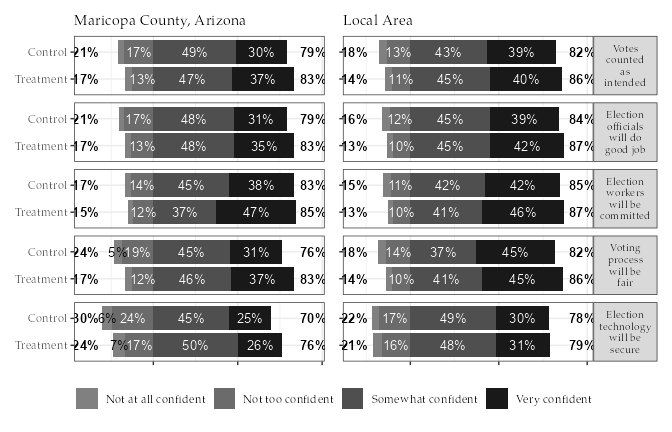
\includegraphics[keepaspectratio]{index_files/figure-latex/notebooks-figures-fig-patch10-output-1.png}}

}

\end{figure}%

Reviewing item responses distinguished by treatment condition reveals
particulars of the treatment effect (Figure~\ref{fig-patch10}). Among
the items that asked about Maricopa County, AZ, it is a bit easier to
see upon which items the treatment vignette had the greatest effect. It
appears that the main effect of the treatment is upon responses to the
item that measures confidence in the security of election technology.

Regarding confidence in the commitment of election staff and volunteers,
a higher proportion of respondents in the treatment group selected
``Very confident'' over ``Somewhat confident'' compared to the control
group, but only for items concerning Maricopa County, AZ. Although
confidence in election workers was generally high across the board, the
shift from ``Somewhat'' to ``Very'' confident for items pertaining to
election worker \emph{commitment} to fairness and accuracy seems to
clearly speak to the group being recruited, i.e., veterans and family
members. However, the same visible shift in proportion from ``Somewhat''
to ``Very'' confident isn't observed when items asked about one's local
area. It may be the case that respondents harbor particular attitudes or
sentiment about Maricopa County, AZ itself, or there may be nothing
uniquely special about Maricopa County, AZ supposing that elections
anywhere beyond one's local area generally garner slightly less
confidence.

What this does suggest, however, is that trust in the fairness and
accuracy of the electoral process is notably higher upon the notion that
military veterans will be directly engaged as election staff and
volunteers in places where such trust falters. The question turns to
whether this also lowers distrust, or the extent to which one expects
electoral fraud to occur.

\begin{figure}[H]

\caption{\label{fig-patch11}Disrust in Election Administration by
Experiment Condition}

\centering{

\pandocbounded{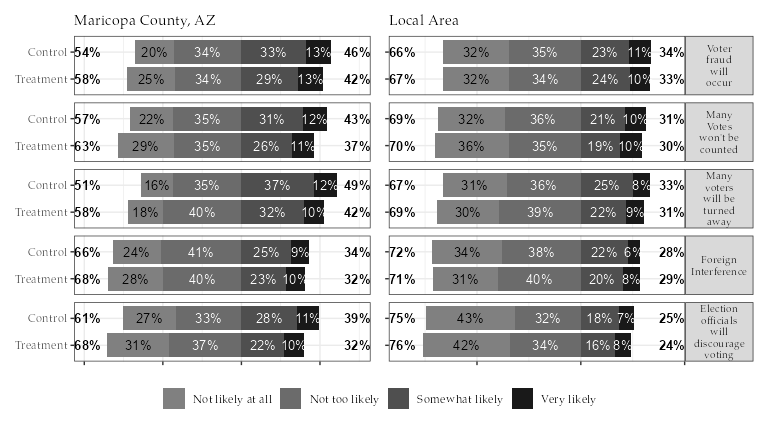
\includegraphics[keepaspectratio]{index_files/figure-latex/notebooks-figures-fig-patch11-output-1.png}}

}

\end{figure}%

Similar to the trust scale items, the items on the distrust scale were
associated with lower distrust in the treatment condition compared to
the control. A quick glance at Figure~\ref{fig-patch11} shows what
appears to be a significant reduction in distrust, especially regarding
the expectations that many votes wouldn't be counted, many voters would
be turned away, and that election officials would discourage voters from
casting a ballot. Interestingly, the expectation that there would be
foreign interference in elections in Maricopa County, AZ were pretty
resilient against the treatment. And again, responses for items
pertaining to elections in one's local area are practically
indistinguishable between treatment and control.

\subsubsection{Confidence in elections}\label{confidence-in-elections}

Once trust and distrust were composed into unified variable of
confidence in elections, I then examined distribution of the dependent
variable followed by analysis of the effect of the treatment by
comparison of mean differences between experiment conditions. Recall
that on this scale, zero reflects insecurity (e.g., similar or equal
values of trust and distrust), whereas values diverging from zero
reflect confidence in either direction, trust or distrust respectively.
Positive values reflect trust in elections administration (e.g.,
elections will be fair and accurate), whereas negative values reflect
distrust in elections (i.e., expectation that election fraud will
occur). To retain a meaningful zero, I rescaled the sum scores to range
from -3 to 3\footnote{This range is mostly arbitrary, as a range from -1
  to 1 works much the same. When relying on simple sum total score, the
  scale ranges from -15 to 15. So a single point increase from 0 to 1
  may reflect a combination of a single ``Very confident'' response on a
  trust item compensated by a single ``Somewhat likely'' response on a
  distrust item (i.e., 3-2 = 1), or some other equivalent combination.
  Although the use of mean scores would place scores back onto the
  response scale metric (e.g., from 0 to 3, reflective of ``not at all''
  to ``very''), this results in a unipolar scale (from 0 to 3). The
  bipolar scale resulting from the composition of positive trust and
  negative distrust engenders meaning to zero and negative values. As
  such, composite mean scores become inappropriate and interpretation of
  scores would no longer be feasible. In other words, negative values on
  the scale for confidence in elections hold substantive meaning (e.g.,
  distrust, absent trust), which makes transforming scores to fit a
  unipolar scale inappropriate.} and then superimposed two histograms of
confidence scores: one derived from AZ items and another for scores
derived from local area items. Doing this is illustrative of the
relative distribution of confidence that differed depending on the
location of elections referred to in the survey items (e.g., Maricopa
County, AZ).

As revealed by review of the item responses, the distribution of
confidence differed depending on whether survey items pertained to
elections in Maricopa County, AZ, or elections within one's local area.

\begin{figure}[H]

\caption{\label{fig-dist}Overlapping Distribution of Confidence in
Elections for AZ and Local Area}

\centering{

\pandocbounded{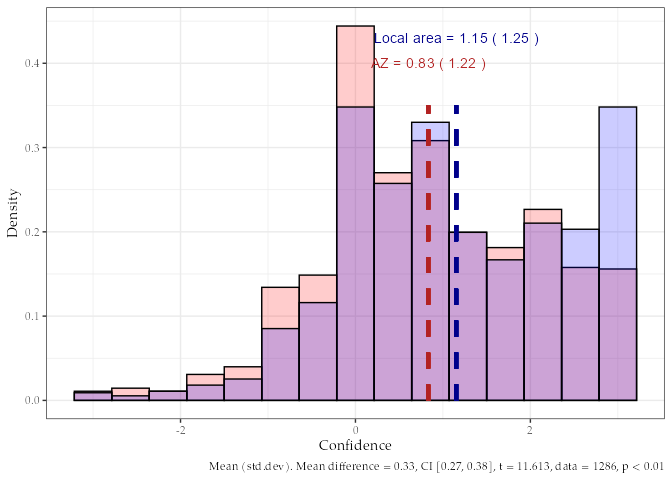
\includegraphics[keepaspectratio]{index_files/figure-latex/notebooks-figures-fig-dist-output-1.png}}

}

\end{figure}%

Overall, the sample expressed more trust in elections relative to
distrust seeing as how the distribution of confidence is largely
positive (Figure~\ref{fig-dist}). However, there's a clear difference
between confidence in Maricopa county, AZ elections and elections within
one's local area. A paired t-test confirms that this difference was
statistically significant, though somewhat small (mean difference
\(= 0.325\), \(95\%\) CI \([0.27, 0.38]\), \(t(1286) = 11.61\),
\(p < .001\)). Nonetheless, respondents appeared less confident
regarding elections in Maricopa County, AZ, but held more confidence in
elections administration in their local area. This complements previous
research that demonstrates a similar bias favorable to one's local area
(\citeproc{ref-stewart2022}{Stewart 2022}).

Accordingly, when confidence levels are distinguished by experiment
condition, the treatment vignette only had an effect upon survey items
pertaining to elections in Maricopa County, AZ. Conducting an
independent samples t-test (i.e., Welch Two Sample t-test) suggests that
the effect of the treatment compared to the control condition is
positive and statistically significant.

\begin{table}[H]

\caption{\label{tbl-ttest}Mean Difference of Treatment Compared to
Control Condition}

\centering{

\centering\begingroup\fontsize{9}{11}\selectfont

\begin{tabular}[t]{llllllllll}
\toprule
Place & $\bar{x}_{diff}$ & $\bar{x}_{treat}$ & $\bar{x}_{control}$ & $treat_{n}$ & $control_{n}$ & t & p & data & CI\\
\midrule
Maricopa County, AZ & 0.20 & 0.93 & 0.72 & 650.00 & 637.00 & 2.96 & 0.003** & 1283.73 & {}[ 0.07, 0.33]\\
Local Area & 0.06 & 1.18 & 1.12 & 650.00 & 637.00 & 0.87 & 0.383 & 1282.95 & {}[-0.08, 0.20]\\
\bottomrule
\multicolumn{10}{l}{\rule{0pt}{1em}\textit{Note: }}\\
\multicolumn{10}{l}{\rule{0pt}{1em}Welch Two Sample t-tests of difference between Confidence in Elections by Treatment Condition.}\\
\end{tabular}
\endgroup{}

}

\end{table}%

The results of Table~\ref{tbl-ttest} show that, on a scale ranging from
-3 to 3, the effect of the treatment is associated with a \(0.20\)
average difference in confidence in elections in Maricopa County, AZ,
compared to the control group. When the dependent variable is centered
to have a mean of \(0\) and standard deviation of \(1\), standardized
parameters permit interpretation of the treatment effect in terms of
standard deviations; the standardized difference in confidence between
treatment and control is \(0.16\) (CI \([0.06, 0.27]\)).

\begin{figure}[H]

\caption{\label{fig-coef1}Confidence in Elections by Experiment
Condition}

\begin{minipage}{\linewidth}

\subcaption{\label{fig-coef1-1}Confidence by Treatment Condition}

\centering{

\pandocbounded{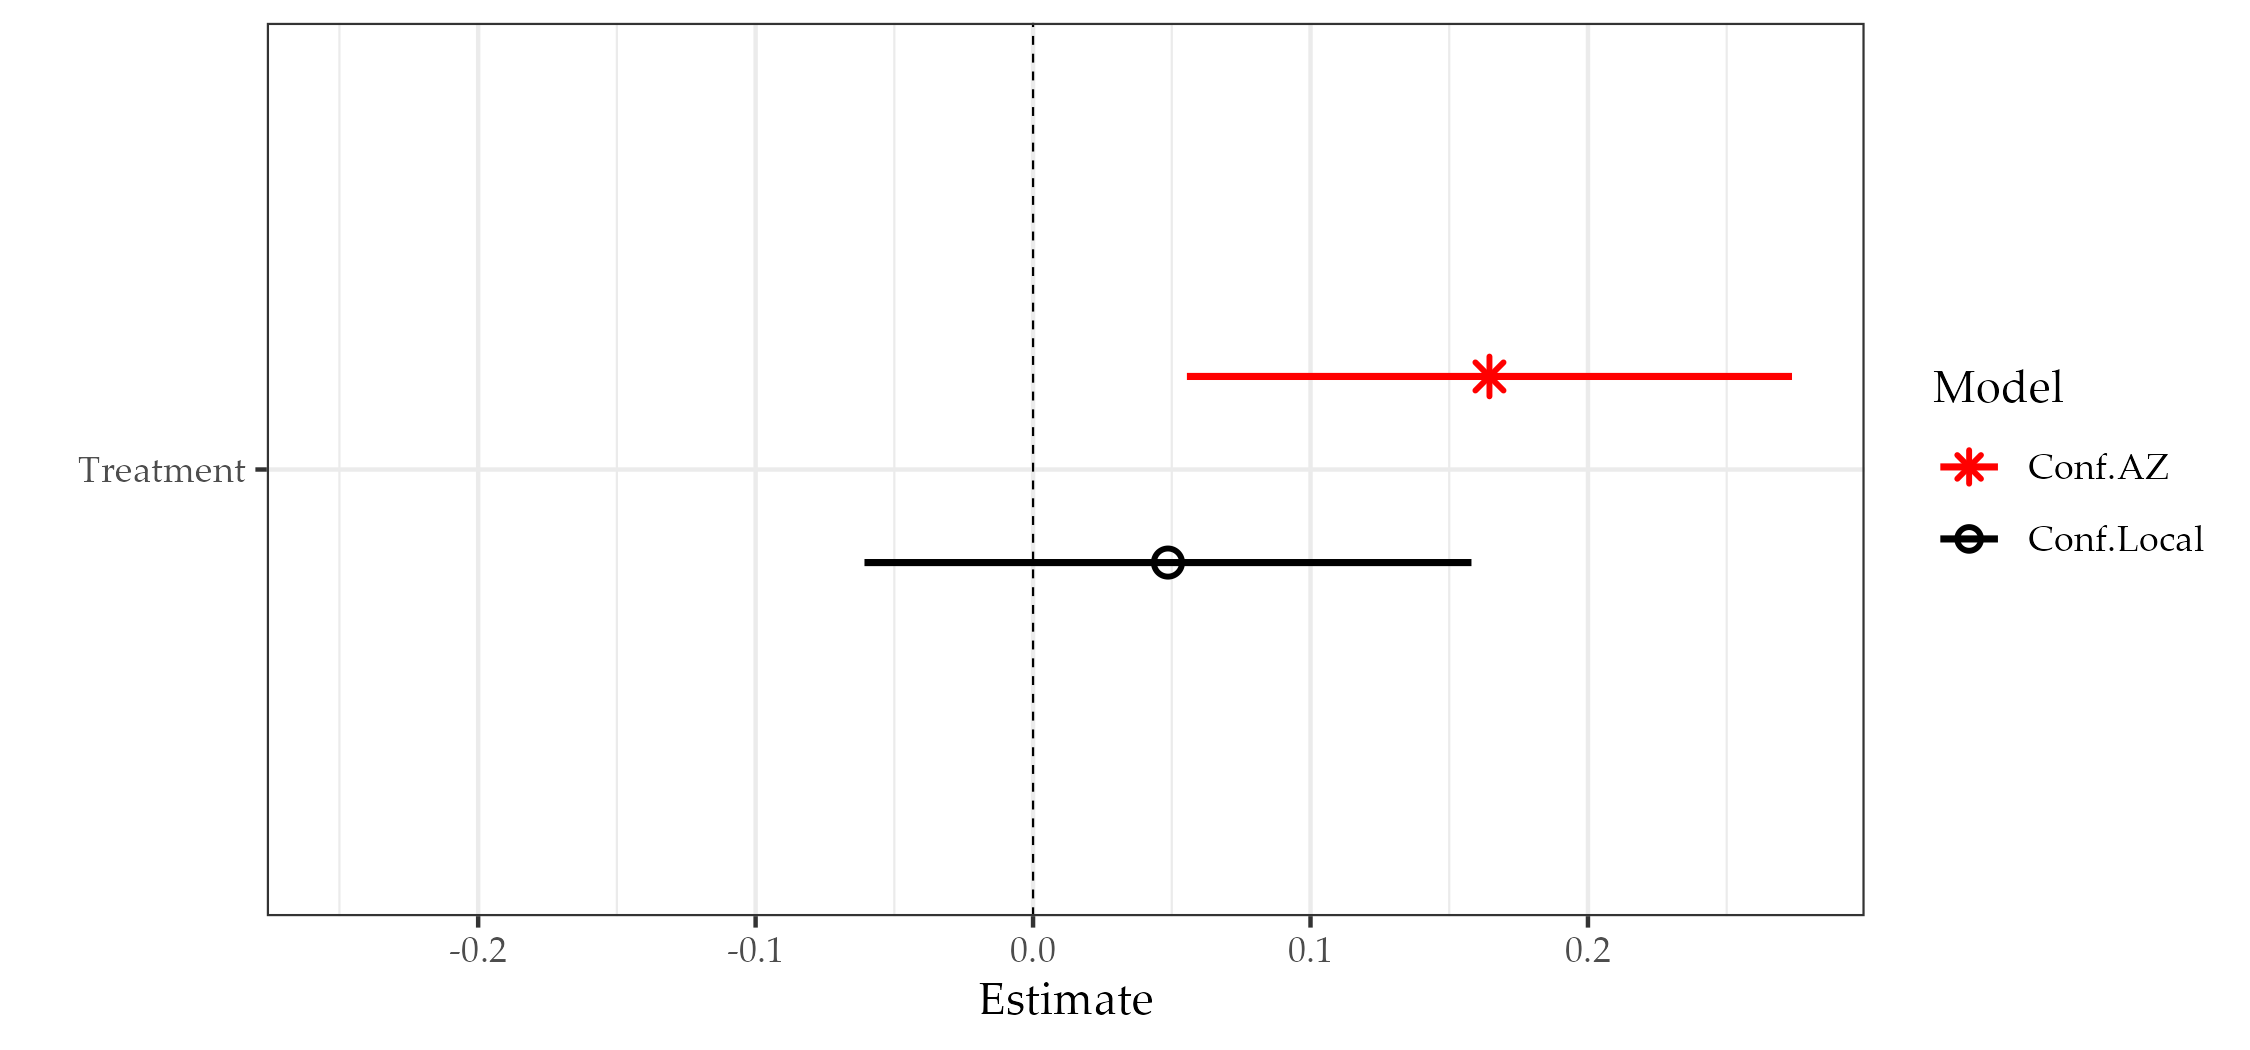
\includegraphics[keepaspectratio]{index_files/figure-pdf/fig-coef1-1.png}}

}

\end{minipage}%
\newline
\begin{minipage}{\linewidth}

\subcaption{\label{fig-coef1-2}Trust and Distrust by Treatment
Condition}

\centering{

\pandocbounded{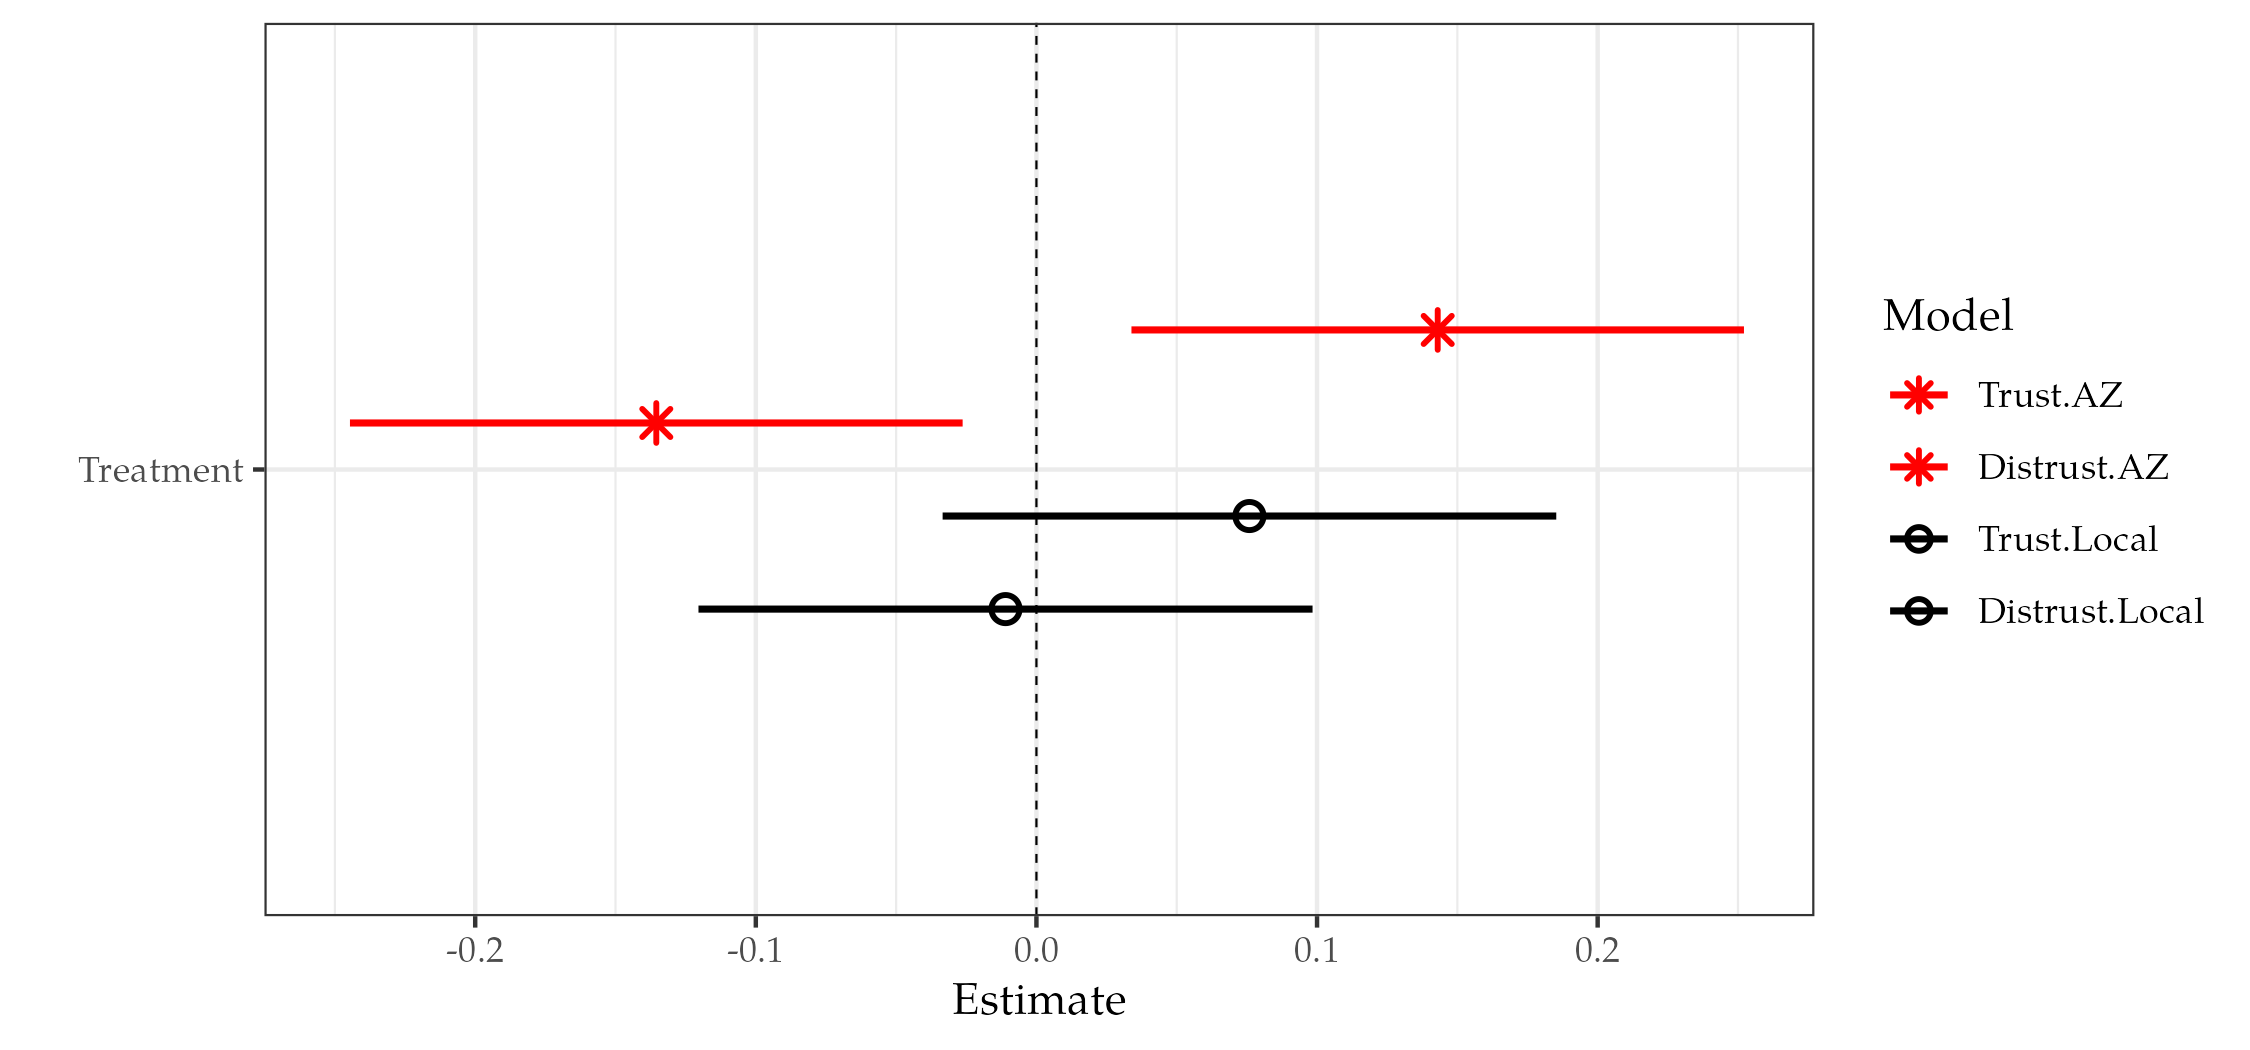
\includegraphics[keepaspectratio]{index_files/figure-pdf/fig-coef1-2.png}}

}

\end{minipage}%

\end{figure}%

Figure~\ref{fig-coef1} displays standard difference estimates of
confidence in elections by treatment condition (control condition as
reference). Figure~\ref{fig-coef1-1} displays two models for confidence
in elections in Maricopa County, AZ, and one's local area by treatment
condition; Figure~\ref{fig-coef1-2} displays the same except
\emph{confidence} is decomposed into its two components, \emph{trust}
and \emph{distrust}. These figures merely illustrate the effect of the
treatment with respect to the relationship between trust and distrust;
ultimately confidence improves.

Confidence in elections was higher among those who read the treatment
vignette but remained conditional on whether the survey questions
inquired about elections in Maricopa County, AZ. This evidence suggests
that announcing efforts to recruit veterans and their families to work
as election staff and volunteers may increase confidence in elections
administration in places outside of one's local area, but may not boost
confidence in elections within one's local area.

\subsubsection{2020 Election Legitimacy
Beliefs}\label{election-legitimacy-beliefs}

I now turn to results examining the effect of the treatment on those who
held onto the belief that the 2020 election results were illegitimate.
First, reviewing responses to items that capture trust in elections, it
is easy to recognize the difference between the way 2020 election
deniers responded with respect to where elections were held.

\begin{figure}[!t]

\caption{\label{fig-patch13}Trust in elections by treatment among those
who refute the 2020 election results}

\centering{

\pandocbounded{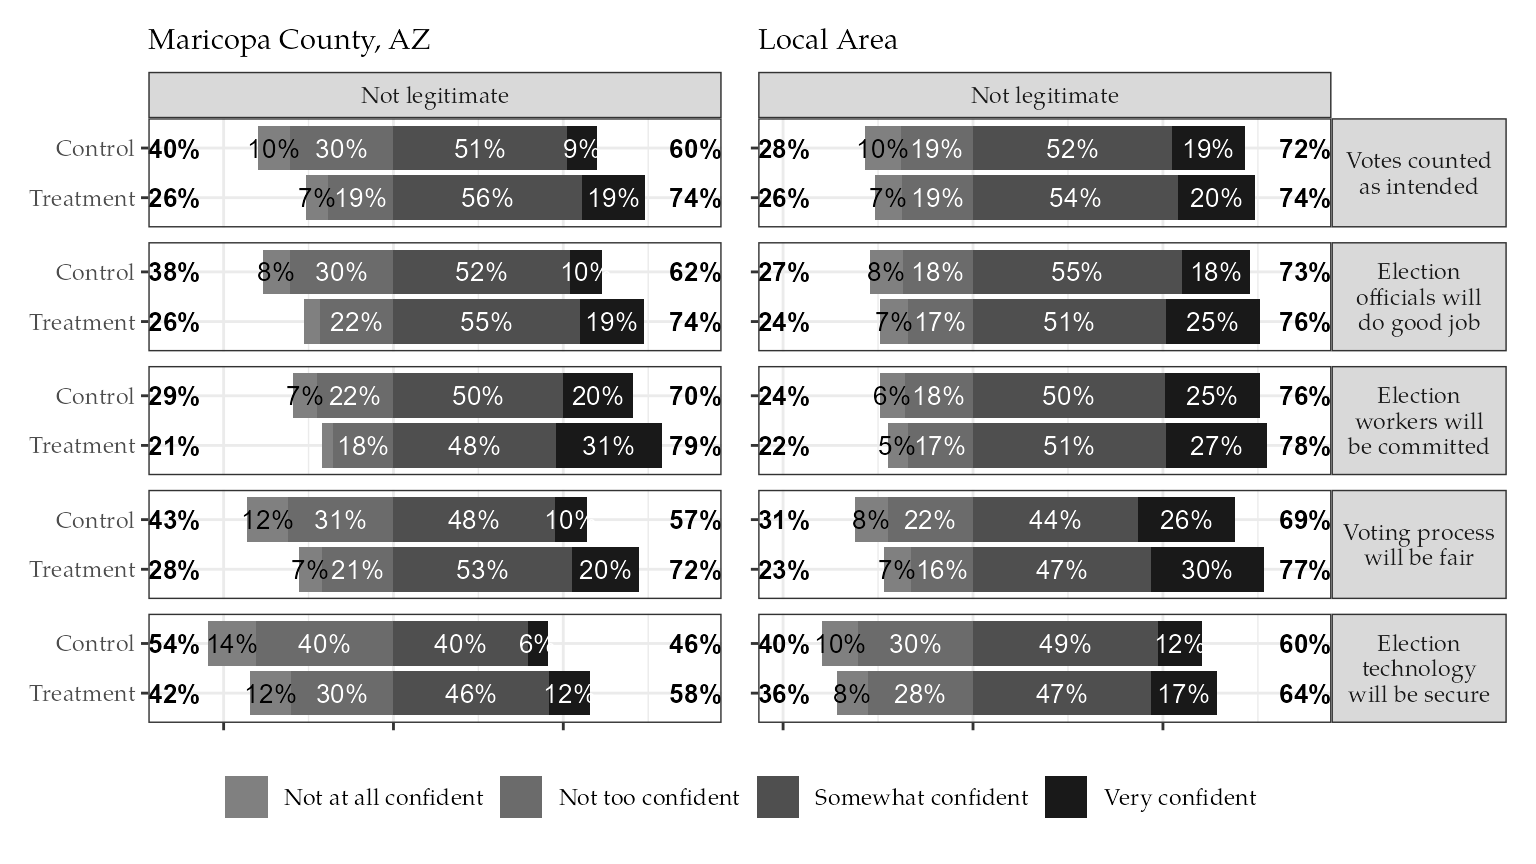
\includegraphics[keepaspectratio]{index_files/figure-latex/notebooks-figures-fig-patch13-output-1.png}}

}

\end{figure}%

Among those who refuted the 2020 election results, trust in Maricopa
County, AZ elections was lower for each item compared to items
pertaining to elections within one's local area, regardless of treatment
condition. However, notably, trust that election technology would be
secure received the lowest confidence endorsement overall. There was
also a notable lack of trust that the voting process would be fair
relative to the other items.\footnote{What is interesting to note here
  is that the first three items regard the more human element of the
  election administration process, e.g., ensuring accuracy of counts,
  competence, and commitment of election workers. Although a neat line
  can't really be drawn between the first three and latter two items
  presented here, it is interesting to see a slight divergence from the
  usual high confidence placed in local area elections.} Now the
comparative difference in responses between those in the treatment group
compared to those in the control group appears substantial for items
pertaining to elections in Maricopa County, AZ.

\begin{figure}[!t]

\caption{\label{fig-patch14}Distrust in elections by treatment among
those who refute the 2020 election results}

\centering{

\pandocbounded{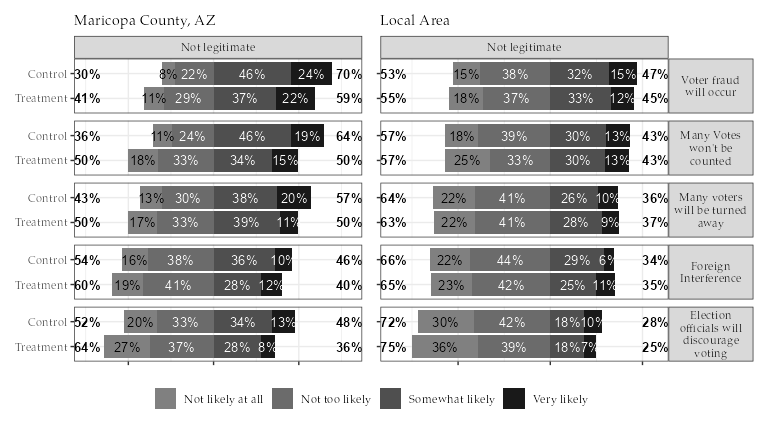
\includegraphics[keepaspectratio]{index_files/figure-latex/notebooks-figures-fig-patch14-output-1.png}}

}

\end{figure}%

Concerning distrust among those who refuted the 2020 election results,
responses items assessing one's expectation that election fraud would
occur reveal the same pattern. Although there is not as stark a
disparity between responses of those in the treatment and those in the
control, among those in the treatment group, there does appear to be
less expectation that election fraud would occur in Maricopa County, AZ.
Overall, review of responses to trust (Figure~\ref{fig-patch13}) and
distrust survey items (Figure~\ref{fig-patch14}) does lend credence to
the impact of the treatment.

In order to substantiate the overall influence of the treatment on
confidence in elections, I regressed the dependent variable confidence
on legitimacy beliefs while controlling for partisanship.

The first model in Table \ref{tbl-legit} shows that overall confidence
in elections among those who read the treatment vignette was
significantly (statistically) greater than those who read the control,
on average and netting out the effects of partisanship and legitimacy
beliefs. Democratic partisanship remains marginally significant at
\(90\%\) confidence level (\(p = 0.055\)). Not believing the 2020
election of Joe Biden was legitimate is negatively associated with
confidence in elections. In order to assess the magnitude of this
interaction effect of the treatment on those who refuted the 2020
election results, I ran a model where confidence in elections was
regressed on the interaction between the treatment and legitimacy
beliefs, controlling for partisanship.

There's a positive interaction effect of the treatment vignette among
those who believe that the 2020 election was not legitimate, on average
and controlling for partisanship. This shows that the treatment effect
was most influential upon those who believe the 2020 election results
were illegitimate. The treatment alone does not reverse such beliefs,
but this shows where its influence was most potent.

\subsection{Conclusion}\label{conclusion}

Publicized announcements that election officials are actively recruiting
former military service members to work as election staff and volunteers
is associated with slightly greater confidence in elections compared to
election worker recruitment announcements that do not explicitly mention
targeted recruitment of former military service members. Moreover,
increased levels of confidence is limited to elections beyond one's
local area and, of course, in anticipation of election night. Whether
the increase in confidence is sustained post-election night cannot be
inferred from these results.

Bear in mind that confidence in elections for one's local area is
already higher than for those beyond. Thus, there's already more
insecurity concerning elections elsewhere for whatever reason. In the
anticipatory period prior to national elections, publicized efforts to
recruit veterans to work as election staff and volunteers may be a
small, but positive, step towards reducing insecurity in elections that
occur elsewhere. Especially among those who maintained a steadataast
degree of distrust in elections. Despite a lack of evidence that
systematic electoral fraud had occurred in the 2020 election, a
substantial proportion of the population were unwilling to affirm the
legitimacy of the results. However, despite such legitimacy beliefs,
most were not consistent as they expressed varying levels of trust in
different aspects of elections administration.

These results speaks more to the influence that military veterans have
among those who distrust the electoral process and refute the legitimacy
of prior outcomes than it does to the public more generally. In general,
public confidence appears strongest when the elections under
consideration regard those within one's local community. Yet, such
strong confidence is not generalized outward to the institution of
elections administration as a whole. Insecurity in the integrity of the
electoral process and its administration may be naturally higher for
elections that occur further from home. Whether that is due to some
local favorability bias or some outward negativity bias is hard to say.
And seeing as how insecurity presents vulnerability, it is perhaps far
easier to inspire a general sense of distrust in the process and its
administration in places not near and around one's local area.

\newpage

\section{Appendix A: Survey Experiment Vignettes and Survey
Items}\label{appendix-a-survey-experiment-vignettes-and-survey-items}

\subsection{Survey Experiment
Vignettes}\label{survey-experiment-vignettes}

\begin{figure}

\begin{minipage}{0.45\linewidth}

\subsubsection{Treatment Vignette}\label{treatment-vignette-1}

\textbf{Local Military Veterans Recruited for Election Jobs in Maricopa
County}\\
\strut \\
\strut ~~PHOENIX (AP) --- Election officials in Maricopa County,
Arizona, announced a program designed to recruit military veterans and
their family members from the community to serve as election
administrators, including election polling place workers, temporary
workers, and full-time staff. As the U.S. general elections in November
near, election officials must fill several thousand temporary positions
and hundreds of other open positions to ensure sufficient staffing for
the 2024 elections and beyond.\\
\strut \\
\strut ~~Army veteran Jordan Braxton just joined the elections
workforce. Jordan believes their role is important to ensuring a secure,
accurate, and transparent election, ``Many places are short on staff
this election cycle. I served my country in the Army, and I want to do
my part as a veteran and a citizen to ensure that everyone trusts the
process and the outcome of the election.''

\end{minipage}%
%
\begin{minipage}{0.10\linewidth}
~\end{minipage}%
%
\begin{minipage}{0.45\linewidth}

\subsubsection{Control Vignette}\label{control-vignette-1}

\textbf{Local Residents Recruited for Election Jobs in Maricopa
County}\\
\strut \\
\strut ~~PHOENIX (AP) ---Election officials in Maricopa County, Arizona,
announced a program to recruit members of the community to serve as
election administrators, including election polling place workers,
temporary workers, and full-time staff. As the U.S. general elections in
November near, election officials must fill several thousand temporary
positions and hundreds of other open positions to ensure sufficient
staffing for the 2024 elections and beyond.\\
\strut \\
\strut ~~Jordan Braxton just joined the elections workforce. Jordan
believes their role is important to ensuring a secure, accurate, and
transparent election, ``Many places are short on staff this election
cycle. I want to do my part as a citizen to ensure that everyone trusts
the process and the outcome of the election.''

\end{minipage}%

\end{figure}%

\newpage

\subsection{Survey Items}\label{survey-items}

\begin{table}

\caption{\label{tbl-4}Survey Items and Response Options}

\centering{

\begingroup\fontsize{8}{10}\selectfont

\begin{tabu} to \linewidth {>{\raggedright\arraybackslash}p{7cm}>{\raggedright\arraybackslash}p{4cm}}
\toprule
Question & response\\
\midrule
In general, how favorable or unfavorable is your impression of local election officials? & {}[Strongly unfavorable, Somewhat unfavorable, Neither, Somewhat favorable, Strongly favorable]\\
\addlinespace
Regardless of whom you supported in the 2020 election, do you think Joe Biden's election as president was legitimate, or was he not legitimately elected? & Legitimate, Not legitimate\\
\addlinespace
Thinking about Maricopa County, AZ, how concerned should voters feel about potential violence, threats of violence, or intimidation while voting in person at their local polling place? & Very concerned, Somewhat concerned, Not too concerned, Not at all concerned\\
\addlinespace
How confident, if at all, are you that in person polling places in Maricopa County, AZ will be safe places for voters to cast their ballots during the upcoming elections in November? & Not at all confident, Not too confident, Somewhat confident, Very confident\\
\bottomrule
\end{tabu}
\endgroup{}

}

\end{table}%

\newpage

\section{Appendix B: Sample Demographics and
Balance}\label{appendix-b-sample-demographics-and-balance}

\subsection{Sample Demographics}\label{sample-demographics}

The median age was 46 (mean age was \(47\)), \(51.7\%\) (\(n = 658\))
women, \(47\%\) (\(n = 598\)) men, and approximately \(1.3\%\) who
identified as either Non-binary/third gender (\(n = 7\)) or preferred
not to say (\(n = 9\)). A large proportion of the sample identified as
White or Caucasian (\(n = 975, 76.65\%\)), while all other non-White
respondents comprised \(27.83\%\) (\(n = 297\)) of the sample. Those who
held a graduate level degree (e.g., Master's, Doctorate, or Professional
level) comprised \(13\%\) of the sample; those with either degree at the
Associate or Bachelor's level comprised \(36.24\%\), while \(22.25\%\)
had some college but no degree; and \(28.46\%\) had either a high school
level or equivalent education or less than high school. The largest
proportion of the sample identified as Democrat at \(44.64\%\), followed
by Republicans at \(42.59\%\). The proportion of true
Independents\footnote{Independent `leaners' were grouped into the
  respective party affiliation in which they lean.} was \(12.78\%\).

\begin{table}

\caption{\label{tbl-demog}Sample Demographics}

\centering{

\centering\begingroup\fontsize{9}{11}\selectfont

\begin{tabular}{lcccc}
\toprule
\textbf{Demographic} & \textbf{N} & \makecell[c]{\textbf{Overall}\ \ \\N = 1,287} & \makecell[c]{\textbf{Control}\ \ \\N = 637} & \makecell[c]{\textbf{Treatment}\ \ \\N = 650}\\
\midrule
\textbf{Age group} & 1,287 &  &  & \\
\hspace{1em}18-34 &  & 350 (27\%) & 170 (27\%) & 180 (28\%)\\
\hspace{1em}35-54 &  & 480 (37\%) & 245 (38\%) & 235 (36\%)\\
\hspace{1em}55-74 &  & 390 (30\%) & 198 (31\%) & 192 (30\%)\\
\hspace{1em}75-85+ &  & 67 (5.2\%) & 24 (3.8\%) & 43 (6.6\%)\\
\addlinespace
\textbf{Gender} & 1,272 &  &  & \\
\hspace{1em}Male &  & 598 (47\%) & 289 (46\%) & 309 (48\%)\\
\hspace{1em}Female &  & 658 (52\%) & 330 (52\%) & 328 (51\%)\\
\hspace{1em}Other/Refused &  & 16 (1.3\%) & 10 (1.6\%) & 6 (0.9\%)\\
\hspace{1em}NA &  & 15 & 8 & \vphantom{4} 7\\
\addlinespace
\textbf{Race/Ethnicity} & 1,272 &  &  & \\
\hspace{1em}White &  & 975 (77\%) & 478 (76\%) & 497 \vphantom{1} (77\%)\\
\hspace{1em}Asian &  & 51 (4.0\%) & 25 (4.0\%) & 26 (4.0\%)\\
\hspace{1em}Black &  & 164 (13\%) & 85 (14\%) & 79 (12\%)\\
\hspace{1em}Other &  & 24 (1.9\%) & 12 (1.9\%) & 12 (1.9\%)\\
\addlinespace
\hspace{1em}Hispanic &  & 44 (3.5\%) & 24 (3.8\%) & 20 (3.1\%)\\
\hspace{1em}American Indian &  & 14 (1.1\%) & 5 (0.8\%) & 9 (1.4\%)\\
\hspace{1em}NA &  & 15 & 8 & \vphantom{3} 7\\
\textbf{White or Non-White} & 1,272 &  &  & \\
\hspace{1em}Non-White &  & 297 (23\%) & 151 (24\%) & 146 (23\%)\\
\addlinespace
\hspace{1em}White &  & 975 (77\%) & 478 (76\%) & 497 (77\%)\\
\hspace{1em}NA &  & 15 & 8 & \vphantom{2} 7\\
\textbf{Education} & 1,272 &  &  & \\
\hspace{1em}H.S. or less &  & 362 (28\%) & 174 (28\%) & 188 (29\%)\\
\hspace{1em}Some college no degree &  & 283 (22\%) & 142 (23\%) & 141 (22\%)\\
\addlinespace
\hspace{1em}College degree &  & 461 (36\%) & 236 (38\%) & 225 (35\%)\\
\hspace{1em}Postgraduate degree &  & 166 (13\%) & 77 (12\%) & 89 (14\%)\\
\hspace{1em}NA &  & 15 & 8 & \vphantom{1} 7\\
\textbf{Party ID} & 1,268 &  &  & \\
\hspace{1em}Independent &  & 162 (13\%) & 83 (13\%) & 79 (12\%)\\
\addlinespace
\hspace{1em}Republican &  & 540 (43\%) & 262 (42\%) & 278 (43\%)\\
\hspace{1em}Democrat &  & 566 (45\%) & 283 (45\%) & 283 (44\%)\\
\hspace{1em}NA &  & 19 & 9 & 10\\
\textbf{Military Relation} & 1,272 &  &  & \\
\hspace{1em}No relation &  & 789 (62\%) & 394 (63\%) & 395 (61\%)\\
\addlinespace
\hspace{1em}Only family &  & 362 (28\%) & 182 (29\%) & 180 (28\%)\\
\hspace{1em}Served w/fam &  & 64 (5.0\%) & 31 (4.9\%) & 33 (5.1\%)\\
\hspace{1em}Served &  & 57 (4.5\%) & 22 (3.5\%) & 35 (5.4\%)\\
\hspace{1em}NA &  & 15 & 8 & 7\\
\bottomrule
\multicolumn{5}{l}{\rule{0pt}{1em}\textsuperscript{1} n (\%)}\\
\multicolumn{5}{l}{\textsuperscript{a} Independents do not identify nor 'lean' toward either political party}\\
\end{tabular}
\endgroup{}

}

\end{table}%

\subsection{Test of Random Assignment to Experiment
Condition}\label{test-of-random-assignment-to-experiment-condition}

Table~\ref{tbl-logit} shows results of a logistic regression test of
random assignment to the treatment group. Demographics such as age,
gender, race, educational attainment, and party ID are included as
predictor variables. Note that 19 missing observations were deleted. A
\(\chi^2(15) = 11.010\), with 15 degrees of freedom and associated
p-value \textgreater{} 0.05 (\(p = 0.75\)) confirms that none of the
demographic predictor variables significantly increased the
log-odds---in turn, the probability---of being assigned to the treatment
group.

\begin{table}

\caption{\label{tbl-logit}Logistic Regression of Random Assignment to
Treatment}

\centering{

\centering\begingroup\fontsize{9}{11}\selectfont

\begin{tabular}{lcccc}
\toprule
  & \textbf{Treatment N} & \textbf{log(OR)} & \textbf{95\% CI} & \textbf{p-value}\\
\midrule
\textbf{(Intercept)} & 640 & 0.17 & -0.25, 0.59 & 0.4\\
\textbf{Age} & 640 &  &  & 0.14\\
\hspace{1em}18-34 & 179 & — & — & \\
\hspace{1em}35-54 & 230 & -0.17 & -0.45, 0.12 & 0.2\\
\hspace{1em}55-74 & 190 & -0.15 & -0.46, 0.15 & 0.3\\
\addlinespace
\hspace{1em}75-85+ & 41 & 0.40 & -0.15, 0.97 & 0.2\\
\textbf{Gender} & 640 &  &  & 0.5\\
\hspace{1em}Male & 308 & — & — & \\
\hspace{1em}Female & 326 & -0.07 & -0.29, 0.15 & 0.5\\
\hspace{1em}Other/Refused & 6 & -0.62 & -1.8, 0.42 & 0.2\\
\addlinespace
\textbf{Race (includes Hispanic as race)} & 640 &  &  & 0.9\\
\hspace{1em}White & 495 & — & — & \\
\hspace{1em}Asian & 26 & 0.03 & -0.55, 0.60 & >0.9\\
\hspace{1em}Black & 79 & -0.08 & -0.43, 0.27 & 0.6\\
\hspace{1em}Other & 11 & 0.05 & -0.82, 0.93 & >0.9\\
\addlinespace
\hspace{1em}Hispanic & 20 & -0.24 & -0.86, 0.38 & 0.5\\
\hspace{1em}American Indian & 9 & 0.50 & -0.58, 1.7 & 0.4\\
\textbf{Educational Attainment} & 640 &  &  & 0.6\\
\hspace{1em}H.S. or less & 188 & — & — & \\
\hspace{1em}Some college no degree & 140 & -0.10 & -0.42, 0.21 & 0.5\\
\addlinespace
\hspace{1em}College degree & 223 & -0.16 & -0.45, 0.12 & 0.3\\
\hspace{1em}Postgraduate degree & 89 & 0.02 & -0.35, 0.40 & >0.9\\
\textbf{Party ID} & 640 &  &  & 0.8\\
\hspace{1em}Independent & 79 & — & — & \\
\hspace{1em}Republican & 278 & 0.12 & -0.24, 0.48 & 0.5\\
\addlinespace
\hspace{1em}Democrat & 283 & 0.05 & -0.31, 0.40 & 0.8\\
\bottomrule
\multicolumn{5}{l}{\rule{0pt}{1em}\textit{Note: }}\\
\multicolumn{5}{l}{\rule{0pt}{1em}Chi-Squared = 11.01, d.f. = 15, p = 0.75}\\
\multicolumn{5}{l}{\rule{0pt}{1em}Abbreviations: CI = Confidence Interval, OR = Odds Ratio}\\
\end{tabular}
\endgroup{}

}

\end{table}%

\newpage

\section{Appendix C: Polychoric Item and Score Correlations of Trust and
Distrust}\label{appendix-c-polychoric-item-and-score-correlations-of-trust-and-distrust}

\subsection{Trust and Distrust}\label{trust-and-distrust}

Polychoric correlation is a measure of association between two ordered
categorical variables each assumed to represent (i.e., indicate, be
influenced by) two normally distributed, continuous, latent variables.
Due to the fact that each item is an ordered categorical variable
assumed to represent one of two latent constructs (i.e., trust or
distrust, respectively), I examined polychoric correlations between the
items used to construct each scale. In addition, one set of the trust
and distrust items pertained to Maricopa County, AZ, whereas the other
set of items were identical except that these items pertained to one's
local area.

Since the two sets of items (AZ items and Local items) are, in theory,
supposed to capture the same normally distributed continuous latent
variables, then the polychoric inter-item correlations should be
significantly associated, strong, and in the same direction for the
items that measure trust regardless of whether the items pertain to AZ
or one's local area (likewise for distrust). Simply, trust/distrust in
elections in AZ should strongly and positively be associated with
trust/distrust in elections in one's local area.

Additionally, the items that indicate trust should negatively correlate
with items that indicate distrust. Furthermore, the strength of the
negative correlations between trust and distrust should closely
approximate if not match.

\phantomsection\label{cell-fig-polycor}
\begin{figure}[h]

\caption{\label{fig-polycor}Polychoric Item Correlation Matrix}

\centering{

\pandocbounded{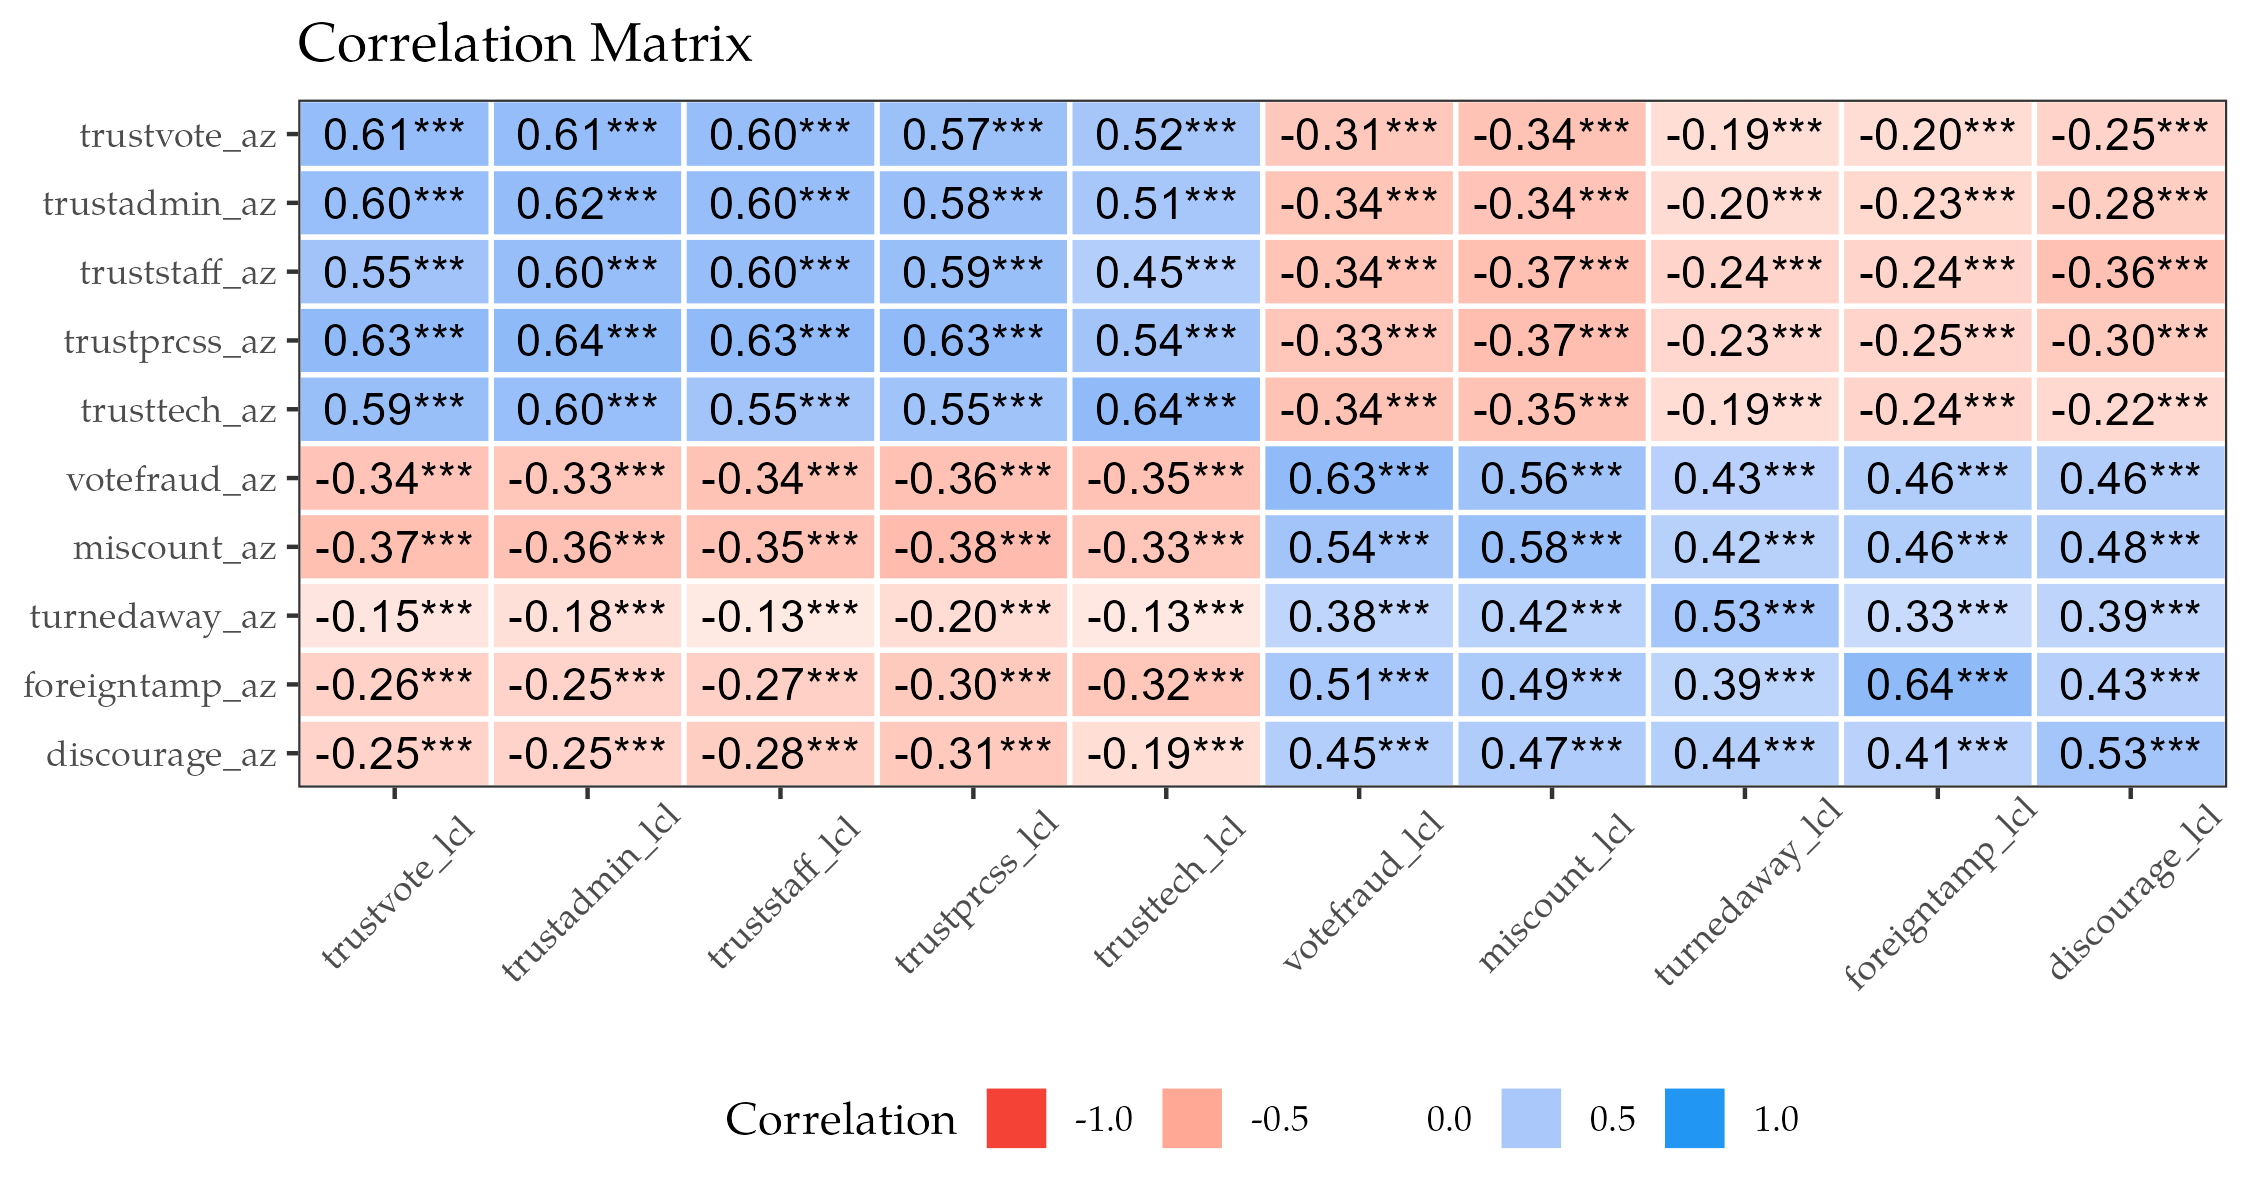
\includegraphics[keepaspectratio]{index_files/figure-pdf/fig-polycor-1.png}}

}

\end{figure}%

Indeed, this is what is revealed by the correlation matrix
(Figure~\ref{fig-polycor}). Trust items correlate positively, strongly,
and are significant regardless of location at which the items pertain.
The same goes for distrust items. Also, items meant to measure trust
negatively correlate with the items that measure distrust. However, the
positive correlations are not nearly as high as would be expected
supposing that the items are nearly identical theoretical indicators of
the same hypothetical constructs, i.e., trust and distrust respectively.

If the items accurately measure trust/distrust in elections regardless
of where those elections are said to take place, then positive
correlations between the AZ and Local area items should approach perfect
correlation as though the same exact questions were asked twice. This
result, however, suggests that the location of which the survey items
pertain (and perhaps other factors) makes a substantial difference in
the pattern of responses, but also raises valid questions as to whether
the items accurately measure the latent variable constructs in the first
place.

Although I do not explicitly assume that the survey instruments
perfectly measure the hypothetical constructs of interest (i.e., trust
and distrust), perfect measurement is implicitly assumed by the method
of combining multiple item responses into a sum or mean composite score.

In short, I expected item responses from the trust and distrust scales
to be inversely correlated among the sample, but not mutually exclusive.
Indeed, this is what I find. Polychoric correlations between the trust
and distrust items negatively correlate as expected, as does the
correlation between the two sum score scales. Given the ordinal nature
of the variable items, I conducted a Spearman's rank correlation test
(\citeproc{ref-spearman1907}{Spearman 1907}) and found a negative
correlation of \(\rho = -0.49\) (\(95\%\) CI {[}-0.53, -0.44{]};
Kendall's \(\tau = -0.39\)) between scores on the two scales for the AZ
items (For the local item scale score correlation: \(\rho = -0.52\),
\(95\%\) CI {[}-0.56, -0.48{]}; Kendall's \(\tau = -0.39\)). The
negative correlation between the trust and distrust items and scores
makes intuitive sense.

\newpage

\section*{References}\label{bibliography}
\addcontentsline{toc}{section}{References}

\phantomsection\label{refs}
\begin{CSLReferences}{1}{1}
\bibitem[\citeproctext]{ref-abbate2020a}
Abbate, Andrea. 2020. {``39 {Ways Election Offices} Are {Responding} to
{COVID-19}.''}
\url{https://www.techandciviclife.org/covid-19-responses/}.

\bibitem[\citeproctext]{ref-atkeson2007}
Atkeson, Lonna Rae, and Kyle L. Saunders. 2007. {``The {Effect} of
{Election Administration} on {Voter Confidence}: {A Local Matter}?''}
\emph{PS: Political Science \& Politics} 40(4): 655--60.
doi:\href{https://doi.org/10.1017/S1049096507071041}{10.1017/S1049096507071041}.

\bibitem[\citeproctext]{ref-bowler2024}
Bowler, Shaun, and Todd Donovan. 2024. {``Confidence in {US Elections
After} the {Big Lie}.''} \emph{Political Research Quarterly} 77(1):
283--96.
doi:\href{https://doi.org/10.1177/10659129231206179}{10.1177/10659129231206179}.

\bibitem[\citeproctext]{ref-brennancenterforjustice2024}
Brennan Center for Justice. 2024. \emph{Local {Election Officials
Survey} --- {May} 2024 \textbar{} {Brennan Center} for {Justice}}.
Brennan Center Research Department.
\url{https://www.brennancenter.org/our-work/research-reports/local-election-officials-survey-may-2024}
(November 5, 2024).

\bibitem[\citeproctext]{ref-carter2024}
Carter, Luke, Ashlan Gruwell, J Quin Monson, and Kelly D Patterson.
2024. {``From {Confidence} to {Convenience}: {Changes} in {Voting
Systems}, {Donald Trump}, and {Voter Confidence}.''} \emph{Public
Opinion Quarterly} 88: 516--35.
doi:\href{https://doi.org/10.1093/poq/nfae034}{10.1093/poq/nfae034}.

\bibitem[\citeproctext]{ref-cikara2014}
Cikara, Mina, and Jay J Van Bavel. 2014. {``The {Neuroscience} of
{Intergroup Relations}.''} \emph{Perspectives on Psychological Science}
9(3): 245--74.

\bibitem[\citeproctext]{ref-claassen2008}
Claassen, Ryan L., David B. Magleby, J. Quin Monson, and Kelly D.
Patterson. 2008. {``{`{At Your Service}'}: {Voter Evaluations} of {Poll
Worker Performance}.''} \emph{American Politics Research} 36(4):
612--34.
doi:\href{https://doi.org/10.1177/1532673X08319006}{10.1177/1532673X08319006}.

\bibitem[\citeproctext]{ref-coll2024a}
Coll, Joseph A, and Christopher J Clark. 2024. {``A {Racial Model} of
{Electoral Reform}: {The Relationship} Between {Restrictive Voting
Policies} and {Voter Confidence} for {Black} and {White Voters}.''}
\emph{Public Opinion Quarterly} 88: 561--84.
doi:\href{https://doi.org/10.1093/poq/nfae032}{10.1093/poq/nfae032}.

\bibitem[\citeproctext]{ref-conde2020}
Conde, Ximena. 2020. {``Philly Area Counties Say Efforts to Recruit Poll
Workers for {Election Day} Are Paying Off.''} \emph{WHYY NPR}.
\url{https://whyy.org/articles/philly-area-counties-say-efforts-to-recruit-poll-workers-for-election-day-are-paying-off/}.

\bibitem[\citeproctext]{ref-cooter2013}
Cooter, Amy. 2013. {``Americanness, {Masculinity}, and {Whiteness}: {How
Michigan Militia Men Navigate Evolving Social Norms}.''} Thesis.
\url{http://deepblue.lib.umich.edu/handle/2027.42/98077}.

\bibitem[\citeproctext]{ref-cooter2024}
Cooter, Amy. 2024. {``Veterans and {Extremism}: {From Militias} to
{January} 6th and {Real Patriots} \textbar{} {Middlebury Institute} of
{International Studies} at {Monterey}.''}
\url{https://www.middlebury.edu/institute/academics/centers-initiatives/ctec/ctec-publications/veterans-and-extremism-militias-january-6th}.

\bibitem[\citeproctext]{ref-corrigan2002}
Corrigan, Patrick W., David Rowan, Amy Green, Robert Lundin, Philip
River, Kyle Uphoff-Wasowski, Kurt White, and Mary Anne Kubiak. 2002.
{``Challenging {Two Mental Illness Stigmas}: {Personal Responsibility}
and {Dangerousness}.''} \emph{Schizophrenia Bulletin} 28(2): 293--309.
doi:\href{https://doi.org/10.1093/oxfordjournals.schbul.a006939}{10.1093/oxfordjournals.schbul.a006939}.

\bibitem[\citeproctext]{ref-daniller2019}
Daniller, Andrew M, and Diana C Mutz. 2019. {``The {Dynamics} of
{Electoral Integrity}: {A Three-Election Panel Study}.''} \emph{Public
Opinion Quarterly} 83(1): 46--67.
doi:\href{https://doi.org/10.1093/poq/nfz002}{10.1093/poq/nfz002}.

\bibitem[\citeproctext]{ref-doubek2024}
Doubek, James. 2024. {``States and Cities Beef up Security to Prepare
for Potential Election-Related Violence.''} \emph{NPR: 2024 Election}.
\url{https://www.npr.org/2024/11/04/nx-s1-5178083/national-guard-police-election-security}
(November 5, 2024).

\bibitem[\citeproctext]{ref-dunn2018}
Dunn, Amina. 2018. {``Elections in {America}: {Concerns Over Security},
{Divisions Over Expanding Access} to {Voting}.''}
\url{https://www.pewresearch.org/politics/2018/10/29/elections-in-america-concerns-over-security-divisions-over-expanding-access-to-voting/}.

\bibitem[\citeproctext]{ref-edlin2024}
Edlin, Ruby, and Lawrence Norden. 2024. {``Poll of {Election Officials
Finds Concerns About Safety}, {Political Interference} \textbar{}
{Brennan Center} for {Justice}.''}
\url{https://www.brennancenter.org/our-work/analysis-opinion/poll-election-officials-finds-concerns-about-safety-political}.

\bibitem[\citeproctext]{ref-ferrer2024}
Ferrer, Joshua, Daniel M Thompson, and Rachel Orey. 2024. \emph{Election
{Official Turnover Rates} from 2000--2024}. Bipartisan Policy Center.
\url{https://bipartisanpolicy.org/download/?file=/wp-content/uploads/2024/04/WEB_BPC_Elections_Admin_Turnover_R01.pdf}.

\bibitem[\citeproctext]{ref-giles2021}
Giles, Ben. 2021. {``Arizona {Recount Of} 2020 {Election Ballots Found
No Proof Of Corruption}.''} \emph{NPR: 2024 Election}.
\url{https://www.npr.org/2021/09/25/1040672550/az-audit}.

\bibitem[\citeproctext]{ref-hall2009}
Hall, Thad E., J. Quin Monson, and Kelly D. Patterson. 2009. {``The
{Human Dimension} of {Elections}: {How Poll Workers Shape Public
Confidence} in {Elections}.''} \emph{Political Research Quarterly}
62(3): 507--22.
doi:\href{https://doi.org/10.1177/1065912908324870}{10.1177/1065912908324870}.

\bibitem[\citeproctext]{ref-hall2007}
Hall, Thad, J. Quin Monson, and Kelly D. Patterson. 2007. {``Poll
{Workers} and the {Vitality} of {Democracy}: {An Early Assessment}.''}
\emph{PS: Political Science \& Politics} 40(4): 647--54.
doi:\href{https://doi.org/10.1017/S104909650707103X}{10.1017/S104909650707103X}.

\bibitem[\citeproctext]{ref-hardy2019}
Hardy, Molly M., Calvin R. Coker, Michelle E. Funk, and Benjamin R.
Warner. 2019. {``Which Ingroup, When? {Effects} of Gender, Partisanship,
Veteran Status, and Evaluator Identities on Candidate Evaluations.''}
\emph{Communication Quarterly} 67(2): 199--220.
doi:\href{https://doi.org/10.1080/01463373.2019.1573201}{10.1080/01463373.2019.1573201}.

\bibitem[\citeproctext]{ref-herndon2020}
Herndon, Astead W. 2020. {``{LeBron James} and a {Multimillion-Dollar
Push} for {More Poll Workers}.''} \emph{The New York Times: U.S.}
\url{https://www.nytimes.com/2020/08/24/us/politics/lebron-james-poll-workers.html}
(November 13, 2024).

\bibitem[\citeproctext]{ref-herrnson2009}
Herrnson, Paul S., Richard G. Niemi, and Michael J. Hanmer. 2009.
\emph{Voting Technology : The Not-so-Simple Act of Casting a Ballot}.
Washington, D.C: Brookings Institution Press.

\bibitem[\citeproctext]{ref-hipes2016}
Hipes, Crosby, Jeffrey Lucas, Jo C. Phelan, and Richard C. White. 2016.
{``The Stigma of Mental Illness in the Labor Market.''} \emph{Social
Science Research} 56: 16--25.
doi:\href{https://doi.org/10.1016/j.ssresearch.2015.12.001}{10.1016/j.ssresearch.2015.12.001}.

\bibitem[\citeproctext]{ref-hooghe2018}
Hooghe, Marc. 2018. {``Trust and {Elections}.''} In \emph{The {Oxford
Handbook} of {Social} and {Political Trust}}, ed. Eric M. Uslaner.
Oxford University Press, 0.
doi:\href{https://doi.org/10.1093/oxfordhb/9780190274801.013.17}{10.1093/oxfordhb/9780190274801.013.17}.

\bibitem[\citeproctext]{ref-jensen2022a}
Jensen, Michael, Elizabeth Yates, and Sheehan Kane. 2022.
\emph{Radicalization in the {Ranks}: {An Assessment} of the {Scope} and
{Nature} of {Criminal Extremism} in the {United States Military}}.
{National Consortium for the Study of Terrorism and Responses to
Terrorism (START): College Park}.
\url{https://www.start.umd.edu/pubs/Radicalization\%20in\%20the\%20Ranks_April\%202022.pdf}.

\bibitem[\citeproctext]{ref-kleykamp2015}
Kleykamp, Meredith, and Crosby Hipes. 2015. {``Coverage of {Veterans} of
the {Wars} in {Iraq} and {Afghanistan} in the {U}.{S}. {Media}.''}
\emph{Sociological Forum} 30(2): 348--68.
doi:\href{https://doi.org/10.1111/socf.12166}{10.1111/socf.12166}.

\bibitem[\citeproctext]{ref-kleykamp2023}
Kleykamp, Meredith, Daniel Schwam, and Gilad Wenig. 2023. \emph{What
{Americans Think About Veterans} and {Military Service}: {Findings} from
a {Nationally Representative Survey}}. RAND Corporation.
\url{https://www.rand.org/pubs/research_reports/RRA1363-7.html}.

\bibitem[\citeproctext]{ref-levendusky2024}
Levendusky, Matthew, Shawn Patterson Jr., Michele Margolis, Yotam Ophir,
Dror Walter, and Kathleen Hall Jamieson. 2024. {``The {Long Shadow} of
the {Big Lie}: {How Beliefs} about the {Legitimacy} of the 2020
{Election Spill Over} onto {Future Elections}.''} \emph{Public Opinion
Quarterly}: nfae047.
doi:\href{https://doi.org/10.1093/poq/nfae047}{10.1093/poq/nfae047}.

\bibitem[\citeproctext]{ref-lincoln2024}
Lincoln, Sophie. 2024. {``Washoe {County} Staff Prepare for {Election
Day}, Announce New Safety Feature at Polls.''}
\url{https://mynews4.com/news/local/washoe-county-staff-prepare-for-election-day-announce-new-safety-feature-at-polls}
(November 5, 2024).

\bibitem[\citeproctext]{ref-loewenson2023}
Loewenson, Irene. 2023. {``Mattis Says Vets at {Jan}. 6 {Capitol} Riot
{`Don't Define the Military'}.''} \emph{Marine Corps Times: name}.
\url{https://www.marinecorpstimes.com/news/your-marine-corps/2023/11/06/mattis-says-vets-at-jan-6-capitol-riot-dont-define-the-military/}.

\bibitem[\citeproctext]{ref-maclean2014}
MacLean, Alair, and Meredith Kleykamp. 2014. {``Coming {Home}:
{Attitudes} Toward {U}.{S}. {Veterans Returning} from {Iraq}.''}
\emph{Social Problems} 61(1): 131--54.
doi:\href{https://doi.org/10.1525/sp.2013.12074}{10.1525/sp.2013.12074}.

\bibitem[\citeproctext]{ref-magni2024}
Magni, Gabriele, and Andrew Reynolds. 2024. {``Candidate {Identity} and
{Campaign Priming}: {Analyzing Voter Support} for {Pete Buttigieg}'s
{Presidential Run} as an {Openly Gay Man}.''} \emph{Political Research
Quarterly} 77(1): 184--98.
doi:\href{https://doi.org/10.1177/10659129231194325}{10.1177/10659129231194325}.

\bibitem[\citeproctext]{ref-maidenberg1996}
Maidenberg, David H. 1996. \emph{Recruiting {Poll Workers}}. Office of
Election Administration, Federal Election Commission.
\url{https://purl.fdlp.gov/GPO/gpo18585}.

\bibitem[\citeproctext]{ref-maricopacountyelectionsdepartment2022}
Maricopa County Elections Department. 2022. \emph{Correcting the
{Record}: {Maricopa County}'s {In-Depth Analysis} of the {Senate
Inquiry}}. Maricopa County, Arizona: {Maricopa County Elections
Department and Office of the Recorder}.
\url{https://elections.maricopa.gov/asset/jcr:a9e03750-0a8f-4162-859f-1d46ac54b485/Correcting\%20The\%20Record\%20-\%20January\%202022\%20Report.pdf}.

\bibitem[\citeproctext]{ref-mcneish2023}
McNeish, Daniel. 2023. {``Psychometric Properties of Sum Scores and
Factor Scores Differ Even When Their Correlation Is 0.98: {A} Response
to {Widaman} and {Revelle}.''} \emph{Behavior Research Methods} 55(8):
4269--90.
doi:\href{https://doi.org/10.3758/s13428-022-02016-x}{10.3758/s13428-022-02016-x}.

\bibitem[\citeproctext]{ref-mcneish2020}
McNeish, Daniel, and Melissa Gordon Wolf. 2020. {``Thinking Twice about
Sum Scores.''} \emph{Behavior Research Methods} 52(6): 2287--2305.
doi:\href{https://doi.org/10.3758/s13428-020-01398-0}{10.3758/s13428-020-01398-0}.

\bibitem[\citeproctext]{ref-mena2020}
Mena, Kelly. 2020. {``States Scramble to Recruit Thousands of Poll
Workers Amid Pandemic Shortage \textbar{} {CNN Politics}.''}
\url{https://www.cnn.com/2020/08/13/politics/poll-worker-shortage-2020-election/index.html}.

\bibitem[\citeproctext]{ref-milton2021}
Milton, Daniel, and Andrew Mines. 2021. \emph{{``{This} Is {War}:''}
{Examining Military Experience Among} the {Capitol Hill Siege
Participants}}. George Washington University.
doi:\href{https://doi.org/10.4079/poe.04.2021.00}{10.4079/poe.04.2021.00}.

\bibitem[\citeproctext]{ref-nadeau1993}
Nadeau, Richard, and André Blais. 1993. {``Accepting the {Election
Outcome}: {The Effect} of {Participation} on {Losers}' {Consent}.''}
\emph{British Journal of Political Science} 23(4): 553--63.
doi:\href{https://doi.org/10.1017/S0007123400006736}{10.1017/S0007123400006736}.

\bibitem[\citeproctext]{ref-nadeem2024}
Nadeem, Reem. 2024. {``Harris, {Trump Voters Differ Over Election
Security}, {Vote Counts} and {Hacking Concerns}.''}
\url{https://www.pewresearch.org/politics/2024/10/24/harris-trump-voters-differ-over-election-security-vote-counts-and-hacking-concerns/}
(November 5, 2024).

\bibitem[\citeproctext]{ref-nevadasecretaryofstate2023}
Nevada Secretary of State. 2023. {``Governor {Joe Lombardo}, {Secretary}
of {State Francisco V}. {Aguilar} Sign {Election Worker Protection Bill}
into Law.''}
\url{https://www.nvsos.gov/sos/Home/Components/News/News/3368/309?backlist=\%2Fsos}
(November 5, 2024).

\bibitem[\citeproctext]{ref-nflfootballoperations2022}
NFL Football Operations. 2022. {``Vet the {Vote}.''}
\url{https://operations.nfl.com/inside-football-ops/social-justice/vet-the-vote/}.

\bibitem[\citeproctext]{ref-pape2024}
Pape, Robert A., Keven G. Ruby, Kyle D. Larson, and Kentaro Nakamura.
2024. {``Understanding the {Impact} of {Military Service} on {Support}
for {Insurrection} in the {United States}.''} \emph{Journal of Conflict
Resolution}: 00220027241267216.
doi:\href{https://doi.org/10.1177/00220027241267216}{10.1177/00220027241267216}.

\bibitem[\citeproctext]{ref-powerthepolls2020}
Power the Polls. 2020. {``Power {The Polls Launches First-of-its-Kind
Effort} to {Recruit New Wave} of {Poll Workers} for {Election Day}.''}
\url{https://www.powerthepolls.org/press-release-2020-06-30}.

\bibitem[\citeproctext]{ref-robitzsch2020}
Robitzsch, Alexander. 2020. {``Why {Ordinal Variables Can} ({Almost})
{Always Be Treated} as {Continuous Variables}: {Clarifying Assumptions}
of {Robust Continuous} and {Ordinal Factor Analysis Estimation
Methods}.''} \emph{Frontiers in Education} 5.
doi:\href{https://doi.org/10.3389/feduc.2020.589965}{10.3389/feduc.2020.589965}.

\bibitem[\citeproctext]{ref-ross2020}
Ross, Doug. 2020. {``Porter {County} Election Officials Recruit Students
to Work Polls.''} \emph{nwitimes.com}.
\url{https://www.nwitimes.com/news/local/porter/porter-newsletter/porter-county-election-officials-recruit-students-to-work-polls/article_b2f1aaf8-1e5f-550e-bbbe-113dcb679f7e.html}.

\bibitem[\citeproctext]{ref-sances2015}
Sances, Michael W., and Charles Stewart. 2015. {``Partisanship and
Confidence in the Vote Count: {Evidence} from {U}.{S}. National
Elections Since 2000.''} \emph{Electoral Studies} 40: 176--88.
doi:\href{https://doi.org/10.1016/j.electstud.2015.08.004}{10.1016/j.electstud.2015.08.004}.

\bibitem[\citeproctext]{ref-spearman1907}
Spearman, Charles. 1907. {``Demonstration of {Formulæ} for {True
Measurement} of {Correlation}.''} \emph{The American Journal of
Psychology} 18(2): 161--69.
doi:\href{https://doi.org/10.2307/1412408}{10.2307/1412408}.

\bibitem[\citeproctext]{ref-steinhauer2020}
Steinhauer, Jennifer. 2020. {``Veterans {Fortify} the {Ranks} of
{Militias Aligned With Trump}'s {Views}.''} \emph{The New York Times:
U.S.}
\url{https://www.nytimes.com/2020/09/11/us/politics/veterans-trump-protests-militias.html}.

\bibitem[\citeproctext]{ref-stewart2022}
Stewart, Charles, III. 2022. {``Trust in {Elections}.''} \emph{Daedalus}
151(4): 234--53.
doi:\href{https://doi.org/10.1162/daed_a_01953}{10.1162/daed\_a\_01953}.

\bibitem[\citeproctext]{ref-vanbavel2021}
Van Bavel, Jay J., and Dominic J. Packer. 2021. \emph{The Power of Us :
Harnessing Our Shared Identities to Improve Performance, Increase
Cooperation, and Promote Social Harmony}. First edition. New York:
Little, Brown Spark.

\bibitem[\citeproctext]{ref-wang2013}
Wang, Lihshing Leigh, Amber S. Watts, Rawni A. Anderson, and Todd D.
Little. 2013. {``Common {Fallacies} in {Quantitative Research
Methodology}.''} In \emph{The {Oxford Handbook} of {Quantitative
Methods} in {Psychology}: {Vol}. 2: {Statistical Analysis}}, ed. Todd D.
Little. Oxford University Press, 0.
doi:\href{https://doi.org/10.1093/oxfordhb/9780199934898.013.0031}{10.1093/oxfordhb/9780199934898.013.0031}.

\bibitem[\citeproctext]{ref-wetheveterans2022}
We The Veterans. 2022. {``Launch of {Vet} the {Vote}.''}
\url{https://vetthe.vote/blogs/news/launch-of-vet-the-vote}.

\bibitem[\citeproctext]{ref-widaman2022}
Widaman, Keith F., and William Revelle. 2022. {``Thinking Thrice about
Sum Scores, and Then Some More about Measurement and Analysis.''}
\emph{Behavior Research Methods} 55(2): 788--806.
doi:\href{https://doi.org/10.3758/s13428-022-01849-w}{10.3758/s13428-022-01849-w}.

\bibitem[\citeproctext]{ref-widaman2024}
Widaman, Keith F., and William Revelle. 2024. {``Thinking {About Sum
Scores Yet Again}, {Maybe} the {Last Time}, {We Don}'t {Know}, {Oh No} .
. .: {A Comment} On.''} \emph{Educational and Psychological Measurement}
84(4): 637--59.
doi:\href{https://doi.org/10.1177/00131644231205310}{10.1177/00131644231205310}.

\bibitem[\citeproctext]{ref-wire2024}
Wire, Sarah D., Phillip M. Bailey, Mary Jo Pitzl, Trevor Hughes, Erik
Pfantz, John Wisely, and Deborah Barfield Berry. 2024. {``Counting Votes
Is Now a Dangerous Job: How It Feels for Frontline, Swing-State
Workers.''}
\url{https://www.usatoday.com/story/news/politics/elections/2024/10/28/election-workers-2024-hostility/75586254007/}
(November 5, 2024).

\bibitem[\citeproctext]{ref-xiao2016}
Xiao, Y. Jenny, Géraldine Coppin, and Jay J. Van Bavel. 2016.
{``Perceiving the {World Through Group-Colored Glasses}: {A Perceptual
Model} of {Intergroup Relations}.''} \emph{Psychological Inquiry} 27(4):
255--74. \url{https://www.jstor.org/stable/26159704} (October 26, 2024).

\bibitem[\citeproctext]{ref-xiao2012}
Xiao, Y. Jenny, and Jay J. Van Bavel. 2012. {``See {Your Friends Close}
and {Your Enemies Closer}: {Social Identity} and {Identity Threat Shape}
the {Representation} of {Physical Distance}.''} \emph{Personality and
Social Psychology Bulletin} 38(7): 959--72.
doi:\href{https://doi.org/10.1177/0146167212442228}{10.1177/0146167212442228}.

\end{CSLReferences}




\end{document}
